\documentclass[]{article}

\PassOptionsToPackage{unicode=true}{hyperref} % options for packages loaded elsewhere
\PassOptionsToPackage{hyphens}{url}

\usepackage[a4paper, margin=1in]{geometry}
\usepackage{lmodern}
\usepackage{amssymb,amsmath}
\usepackage{ifxetex,ifluatex}
\usepackage{fixltx2e} % provides \textsubscript
\ifnum 0\ifxetex 1\fi\ifluatex 1\fi=0 % if pdftex
  \usepackage[T1]{fontenc}
  \usepackage[utf8]{inputenc}
  \usepackage{textcomp} % provides euro and other symbols
\else % if luatex or xelatex
  \usepackage{unicode-math}
  \defaultfontfeatures{Ligatures=TeX,Scale=MatchLowercase}
\fi
% use upquote if available, for straight quotes in verbatim environments
\IfFileExists{upquote.sty}{\usepackage{upquote}}{}
% use microtype if available
\IfFileExists{microtype.sty}{%
\usepackage[]{microtype}
\UseMicrotypeSet[protrusion]{basicmath} % disable protrusion for tt fonts
}{}
\IfFileExists{parskip.sty}{%
\usepackage{parskip}
}{% else
\setlength{\parindent}{0pt}
\setlength{\parskip}{6pt plus 2pt minus 1pt}
}
\usepackage{hyperref}
\hypersetup{
            pdftitle={Machine Learning, Architectural Styles and Property Values},
            pdfauthor={Thies Lindenthal* (University of Cambridge) \& Erik B. Johnson (University of Alabama)},
            pdfborder={0 0 0},
            breaklinks=true}
\urlstyle{same}  % don't use monospace font for urls
\setlength{\emergencystretch}{3em}  % prevent overfull lines
\providecommand{\tightlist}{%
  \setlength{\itemsep}{0pt}\setlength{\parskip}{0pt}}
\setcounter{secnumdepth}{0}
% Redefines (sub)paragraphs to behave more like sections
\ifx\paragraph\undefined\else
\let\oldparagraph\paragraph
\renewcommand{\paragraph}[1]{\oldparagraph{#1}\mbox{}}
\fi
\ifx\subparagraph\undefined\else
\let\oldsubparagraph\subparagraph
\renewcommand{\subparagraph}[1]{\oldsubparagraph{#1}\mbox{}}
\fi

% set default figure placement to htbp
\makeatletter
\def\fps@figure{htbp}
\makeatother

\usepackage{soul}
\usepackage{color}
\sethlcolor{yellow}
\usepackage{float}
\usepackage{booktabs}
\usepackage{graphicx}
\usepackage{grffile}
\usepackage{bm}
\usepackage{amsmath}
\usepackage{setspace}
\usepackage{multirow}
\doublespacing
\usepackage[backend=bibtex, style=authoryear]{biblatex}
\usepackage[]{biblatex}
\addbibresource{bibliography.bib}

\begin{document}

\title{Machine Learning, Architectural Styles and Property Values}
\author{Thies Lindenthal* (University of Cambridge) \& Erik B. Johnson
(University of Alabama)}
\date{7 November 2020}

\maketitle
\begin{abstract}
This paper couples a traditional hedonic model with architectural style classifications from human experts and machine learning (ML) enabled classifiers to estimate sales price premia over architectural styles, both at the building and the neighborhood-level. We find statistically and economically significant price differences for houses from distinct architectural styles across an array of specifications and modeling assumptions. Comparisons between classifications from ML models and human experts illustrate the conditions under which ML classifiers may perform at least as reliable as human experts in mass appraisal models. Hedonic estimates illustrate that the impact of architectural style on price is attenuated by properties with less well-defined styles and we find no evidence for differential price effects of \emph{Revival} or \emph{Contemporary} architecture for new construction.
\end{abstract}

\let\svthefootnote\thefootnote
\let\thefootnote\relax

\footnote{{*Corresponding author: Thies Lindenthal (htl24@cam.ac.uk). Replication files are available from the author's Github repository \href{https://github.com/thies}{https://github.com/thies}. Paul E. Glade and Lukas Heckmann-Umhau are thanked for their exceptional research assistance. Carolin Schmidt, Peter Brummund, Mike Langen, Colin Lizieri, Franz Fuerst, Stanimira Milcheva, D'Maris Coffman, Norm Miller, Stephen Malpezzi, John Clapp, Pavel Krivenko and participants at the ASSA/AREUEA 2019 annual meeting and seminars at UCL/Bartlett and the Homer Hoyt Institute offered excellent feedback and critique on earlier versions of this paper.}}

\addtocounter{footnote}{-1}\let\thefootnote\svthefootnote

\newpage

\hypertarget{introduction}{%
\section{Introduction}\label{introduction}}
In this paper, we introduce a new data collection technique that allows us to rigorously test the notion that households have strong preferences over architectural styles. Our results indicate that 1) there is evidence for sales price premia associated with houses from a variety of architectural styles, 2) hedonic estimates from high confidence machine learning (ML) enabled architectural image classifications are similar to human expert estimates, and 3) any style premia are found for existing structures only and not for new buildings, indicating that debates about strong demand for historicizing aesthetics may be unfounded.  

Understanding household preferences for architectural styles is of increasing interest to both policymakers and researchers. The policy perspective is best illustrated by Britain's \emph{Building Better, Building Beautiful Commission}, which advises the government on design choices for homes and neighborhoods. It lists as one of its primary aims as \emph{``To make the planning system work in support of better design and style, not against it.''} \autocite{economistlineofbeauty2018} and boldly claims that matching the style of new housing to aggregate neighborhood preferences should overcome otherwise prevailing objections of incumbent households to new construction.

Researchers have recently begun to quantify and define what makes for \emph{better design and style}. \textcite{Buitelaar2017} find evidence on the link between preferences over architectural styles and housing prices using architectural assessments by human experts, and estimate a sizable premium of 5\% for new buildings in the Netherlands that refer to traditional styles and a staggering 15\% premium for new buildings that closely follow traditional shapes, facade composition, and details. \textcite{Coulson2008} suggest a non-parametric estimator and establish a U-shaped age function and distinct price discounts for postwar and contemporary styles (vis-à-vis more historic styles). \textcite{Francke2017a} investigate the depreciation of residential real estate in The Netherlands and decompose land versus structure values singling out the effect of physical deterioration, functional obsolescence, and vintage effects. They find that buildings from the 1930s carry a strong price premium. These results support the hypothesis that preferences for house vintages (which coincide with architectural styles) may affect housing prices.

Clearly, building vintage, quality, location, and architectural styles are highly correlated which implies that hedonic price estimates for architectural styles cannot simply be understood as marginal prices for aesthetics. We only interpret our empirical findings as `pure' architectural preferences in few cases where differences in all other dimensions can be accounted for, e.g. new units at similar locations that have been built to similar standards and that have not depreciated yet. For markets with more contemporary housing stocks, differences in functional obsolescence would be a major concern when age and style variables are correlated. In our case, over 93\% of the housing stock had been produced prior to 1980 and 70\% before 1940,  so concerns on contemporaneous depreciation of new structures may be alleviated as the vast majority of homes has already depreciated. Nevertheless, systematic differences in locations and unobservable quality characteristics and modernization standards cannot be ruled out.

\textcite{Buitelaar2017} indicate that any premium for an architectural style must stem from either differences in construction prices or from supply
constraints, as new construction potentially does not capture the demand
for traditional styles. In markets where home builders are free to decide on the architectural style of the homes they supply, we would not expect any price effects beyond differences in construction costs. If there was, for instance, a premium for more traditional styles, developers would continue to build more of these until all demand is met. Our prior is therefore \emph{not} to find distinct price effects of aesthetics for newly supplied homes. 

Of course, residential buildings rarely stand in isolation and \textcite{Ahlfeldt2012} investigate the influence a building's architecture exerts on its surroundings. They observe a positive price effect for residential buildings in the direct proximity of iconic homes by Frank Lloyd Wright in Oak Park, Illinois. A building's exterior does not need to be an architectural masterpiece to co-determine the value of other houses close by. A similarly shaped neighboring building is value-enhancing while proximity to a wildly different neighboring shape, everything else remaining equal, may be detrimental to property values \autocite{Lindenthal2017b}. 

In traditional approaches chosen by e.g.~\textcite{Buitelaar2017} or \textcite{Ahlfeldt2012}, each observation is classified into an architectural style by a human expert, which is time-consuming, costly and is not feasible for large sample sizes. As \textcite{Helbich2013} state, the benefit of using new methods to observe the built environment is that ``essential determinants influencing real estate prices {[}which{]} are constantly missing and are not accessible in official and mass appraiser databases''. This is certainly the case in our context, as understanding the impact of architectural style on housing prices is made difficult by the paucity of sales or assessment data that includes architectural style as a characteristic. In addition, an expert's views may not fully reflect the market's perceptions of relevant styles -- architectural classifications and economically relevant segments might differ.

Combining automated Google Street View photo data collection with deep learning/ML image classification offers a promising way forward to large and comprehensive data sets of architectural style. \textcite{Naik2017} describe how neighborhood demographics may impact the physical appearance of neighborhoods. \textcite{Gebru2017} use classified vehicle make and model information to predict income, race, education, and voting patterns at the precinct level. \textcite{Glaeser2016} predict income in New York City. \textcite{Naik2016AER} create a neighborhood safety based Streetscore which is shown to be highly correlated with neighborhood population
density and household income. \textcite{Nadai2016} find that greenery
and street-facing windows contribute to a positive appearance of safety
while \textcite{Liu2017} evaluate the quality and upkeep of the built
environment along Beijing's streets. 

In contrast to the block, street, or street-section level classifications used in the majority of previous studies that use automated image classification, \textcite{GlaeserKincaidNaik2018} push the level of observation to the individual \emph{building level}. Utilizing images of buildings' exteriors collected from Google Street View\footnote{\href{https://www.google.co.uk/maps}{https://www.google.co.uk/maps}}, and to a lesser degree interior images from Zillow, they find that looks matter, at least in Boston: A one standard deviation improvement of a building's exterior is associated with an additional USD 70,000 in home value. Intuitively, the link between good looks and value is
bi-directional: The appearance of buildings that went through foreclosure deteriorated significantly \autocite{GlaeserKincaidNaik2018}.

We follow the framework used by \textcite{GlaeserKincaidNaik2018} and focus on individual buildings as our unit of observation. This focus unlocks one of the main benefits of using mass collected street-level imagery in economic research: property characteristics previously deemed ``unobservable'' can be directly observed in an increasingly accurate and objective manner and may be implemented in a more efficient, accessible, and cost-effective way. 

In addition to reducing the cost of data collection, the ability for low-cost classification of a large sample of structures in an urban area enables researchers to detect not only the architectural style of the building but also to characterize the style of other buildings in the vicinity. This allows us to examine the interaction between the style of a building and that of its neighbors. 

To analyze the accuracy of our method of detecting architectural style, we compare our algorithmic results with an extensive data set of architectural style classifications compiled by human experts. The relatively large and costly comparison group provides insights into ML-based classification accuracy and the robustness of hedonic estimates to human and ML classifications. In addition, the measurable uncertainty in the ML classifications may also be a useful source of variation to exploit for style identification.  For example, it may be the case that the impact of architectural style on sales price for existing buildings may be attenuated for buildings that are more difficult to classify. To our knowledge, this step is not present in the existing literature and provides additional insight into the efficacy of the technique for application in other domains.

 We find evidence that for existing buildings, the architectural style has an impact on the sales price and that the estimates are very similar for both human expert and high confidence ML classified images. The price effects of human-expert defined architectural styles are greater in images where there is agreement with the ML classifications. The presence of architectural style in our hedonic specifications reduces the RMSE of our models. The preferred architectural style for resales appears to be \emph{Revival} with \emph{Interwar}, \emph{Postwar}, and \emph{Early Victorian} commanding the smallest premium. Immediately proximate neighbor styles also have an impact on sales price, with Contemporary neighborhoods clearly preferred to Georgian, Early Victorian, and Postwar. Importantly for policymakers, we do not identify a premium for either Revival or Contemporary styles for new construction. 
 
We begin by describing the traditional hedonic data used in the paper. Second, we describe the methodology for the automated architectural style classification. Third, we compare the results of the automated predictions with expert classifications. Next, we present an array of hedonic regressions using both architect and ML-based classification and discuss results. Finally, we conclude with a discussion of the policy implications of the estimates and the feasibility of ML-based classification of architectural style. 

\hypertarget{Data}{%
\section{Data}\label{data}
}

Residential real estate transactions in England and Wales are
collected and published by the Land Registry
\autocite{LandRegistry2016a}. Their records include the date of transaction, the price paid, street address, a classification of the
property type (flat, detached, semi-detached, or terraced house), the
estate type (freehold or leasehold), and an indicator for newly built
properties. We select transactions from Cambridge, England, which were recorded
between January 1995 and October 2018, excluding any leaseholds, apartments
and properties classified as type ``other'', and sales with prices below
£50,000 or in excess of £2,000,000. Notably, the Land Registry data lack relevant variables such as year of construction, home and lot size, or similar quality indicators. We, therefore, augment the transaction data with core hedonic variables from other sources and to control for a variety of building-specific effects that may be correlated with both sales price and architectural style.

The Ordnance Survey (OS)\footnote{\url{https://www.ordnancesurvey.co.uk/}} provides high-resolution maps that show the two-dimensional footprint of buildings in the UK. Using these maps, we calculate each building's floor plate (in \(m^2\)) and estimate its volume by combining the building outlines with digital elevation models from the \textcite{EnvironmentAgency2015}, as suggested by \textcite{Lindenthal2017}. Additionally, we measure the distance from each residential property to the city center, proxied by Great St.~Mary's Church. The \textcite{ONS2017} subdivides Cambridge into 69 unique \emph{Lower Super Output Areas} (LSOA) and we rely on these boundaries when constructing neighborhood dummy variables. An LSOA typically has 1,000--3,000 residents and 400--1,200 households of comparable economic and socio-demographic characteristics \autocite{ONS2017b}. 


\hypertarget{ml-classification-of-building-styles}{%
\subsection{Architectural Style Data}\label{ml-classification-of-building-styles}}

Our main variable of interest, architectural style, follows the classifications commonly used by realtors, home-buyers, and architects. Styles are distinctive in Cambridge: Table \ref{tab:styles_rubric} provides a description of the construction eras and the distinctive motifs for each style as defined by members of the Architecture Department at the University of Cambridge. 

\begin{center}
  -- Insert Table \ref{tab:styles_rubric} about here --
\end{center}

We aim to collect images of all residential buildings in Cambridge from Street View. Approximately 50,000 buildings found on the OS maps have footprints between 30 and 500 $m^2$. For 85\% of these candidates, we can download street-level images on Google Street View. However, not all of them turn out to be residential buildings. A sample of 25,000 of these images is categorized by final year architecture students into the seven styles. 

 We can match 23,768 residential properties sold in Cambridge between 1995 and 2019 to images from Google Street View. We implicitly assume that houses have not changed their architectural styles between the time of sale and the time Google collected the images. This is a reasonable approach since conversions of just the exterior of buildings rarely occur. In case of full redevelopments, we exclude any sales for that address pre-dating the redevelopment, since we cannot rule out a change of style at redevelopment.
 
 Importantly, 15,511 sales can also be matched to the sample of expert's classifications. Our hedonic models will be estimated on these observations for which we have predicted and ground truth classifications. This allows us to assess the prediction accuracy and robustness of the regression results to the classification approach. When assessing the architectural style of surrounding buildings, we use the full set of all images collected. Being able to cover almost the universe of all buildings in a market is a clear advantage of an automated approach.

In Figure \ref{fig:vint_examples}, we present a set of representative images for each of the 7 architectural styles. These images come from our automated collection procedure and are a visual representation corresponding to the expert descriptions in Table \ref{tab:styles_rubric}. Image information here is very useful as it provides a visual mapping from the style characteristics to actual identification. One component which is evident in the images but not necessarily in the descriptions is the within style homogeneity of window grouping, relative pane size, and counts. For example, Georgian windows contain 12 equally sized panes in 4 rows and 3 columns, Early Victorian windows consist of 4 equally sized panes in 2 rows and 2 columns, Interwar windows contain an upper smaller pane and larger lower pane. Interestingly, the Revival style demonstrates heterogeneous window patterns that borrow from the variety of classic architectural styles. We revisit the impact of image quality and window visibility on prediction accuracy below.


\begin{center}
  -- Insert Figure \ref{fig:vint_examples} about here --
\end{center}

\hypertarget{image-collection}{%
\subsection{Image collection}\label{image-collection}}

To provide the best information to detect style for both the architect and ML classifiers, images should be focused on the structure under examination, have a clear field of view, show minimal picture overlap with neighboring properties, and minimize potentially confounding issues such as  vehicle type.

Unfortunately, in the UK, Google's Street View API regularly fails to identify the building at a given address. Instead, the camera location will be in close proximity to the front of the building but aimed straight ahead and down the center of the road. Fig. \ref{fig:84Vin} (a) presents a typical result from an address level API. Here, the Google Street View API algorithm fails to accurately capture the front of the building and the property is not even contained in the photo. For major US cities, the accuracy of Google's search results is higher and the Street View camera will pan towards the center of the property parcel. This makes the photo collection of studies such in U.S urban areas potentially much more straightforward although the API may result in images that are too 'zoomed out' resulting in images that may contain obstructed views, vehicles, and neighboring properties.

\begin{center}
  -- Insert Figure \ref{fig:84Vin} about here --
\end{center}

Our automated image collection algorithm utilizes a sophisticated process of viewshed analysis based on Ordnance Survey building maps and ML methods to capture images using the best camera locations, zoom, and angles while accounting for potential obstructions from buildings and trees or vehicles. Thus, for each property, our goal is to automate the collection of the best possible Street View image for each property in our sample. 

More specifically, we first use OS maps to identify each building's outline (see Figure \ref{fig:fan}). Second, we build a database of all possible Google Street View camera locations using Metadata queries of addresses in the Ordnance Survey.  These metadata queries return the latitude, longitude, and dates of the most recent panorama photos collected by Google Street View. Next, we use the OS data to assign each property to the nearest Street View photo location in the metadata database and conduct a viewshed analysis on surrounding building outlines to assign pan and zoom parameters to find an informative view. The algorithm allows us to estimate the camera bearing (green line) and zoom factor, based on the fan of the lines of sight (in blue). The line of sight criteria identifies which exterior walls are visible from the nearest Street View point and aims away from any wall segments where the direct line of sight is obstructed by other buildings. A visual example of this algorithm is shown in  Figure \ref{fig:fan}.\footnote{Code necessary to replicate the full image capture including metadata capture and viewshed based camera aiming is available from \url{https://github.com/thies/paper-cambridge-vintages}}. For each property, we then collect the image at the highest resolution offered by Google's Street View API\footnote{\href{https://developers.google.com/maps/documentation/streetview/intro}{https://developers.google.com/maps/documentation/streetview/intro}} (640x640 color pixels). We test the robustness of our hedonic models to a variety of image quality concerns in the results section of the paper.

\begin{center}
  -- Insert Figure \ref{fig:fan} about here --
\end{center}

Figure \ref{fig:84Vin} (b) shows how the suggested approach can improve the quality of the harvested images. The new image is focused appropriately on the relevant property, it contains minimal neighbor information. and the view is not overly obstructed by other structures, greenery, or vehicles. As a result, the image contains the relevant identifying architectural style characteristics such as a clearly identified roofline, front door, window panes, and bay window.


\hypertarget{image-classification}{%
\section{Methodology: Style classification}\label{image-classification}}

With the images collected, we next focus on training an ML learning model to classify the architectural style observed in each of the collected Street View images. The first step in building our ML model is to construct a training data set. Our training data set consists of images from 25,000 randomly sample properties classified into one of seven different architectural styles by final year students from the Architecture Department at the University of Cambridge\footnote{The full set of classified images are available for download at the authors' websites.} A sample of 25,000 is much more training data than is actually needed. By applying transfer learning to an existing image recognition model, we require less than 250 observations per category to reach saturated training accuracy levels. We use this ``surplus'' training data to perform out of sample comparisons between our ML predictions and human expert classifications. This large set of expert classified data also allows us to perform robustness, and falsification checks on the hedonic regressions for the 15,369 overlapping observations where we have transaction data with both human and ML-based style classifications.

\hypertarget{transfer-learning}{%
\subsection{Training the model}\label{transfer-learning}}

We simplify the calibration of our architectural style prediction model by utilizing transfer learning. Transfer learning freezes the parameters from a pre-trained image recognition model, removes the final steps in the model, and then trains a new model on the vector of outputs from the truncated pre-trained model to produce new classifications\footnote{For examples, see \url{https://www.tensorflow.org/tutorials/images/transfer_learning}}. Transfer learning methods enable the use of smaller training data sets and impose a much lower computational burden than traditional deep learning models. 
For our purposes, we use the \emph{Inception-v3} deep convolutional
neural network \autocite{Szegedy2015}. \emph{Inception-v3} has been
trained for the ImageNet Large Scale Visual Recognition Challenge
(ILSVRC)\footnote{\url{http://image-net.org/challenges/LSVRC/}}, which
evaluates image classification and object detection algorithms for a
wide range of objects. The pre-trained classifications would allow us to
identify pets, vehicles, or people in the pictures -- assessing
architectural style, however, is beyond the canned classifiers'
capabilities. To allow for the detection of new objects, transfer learning techniques strip off the last steps of the model. The output of the original deep learning model is essentially just a deeply recursive dimension reduction engine that outputs a 2048-dimensional feature vector for each picture. This feature vector describes the outline shapes, locations, and colors that were important for the ImageNet classifications. 

\textcite{GlaeserKincaidNaik2018} rely on a different ILSVRC competitor, \emph{Resnet-101} \autocite{He2016}. They reduce the extracted feature vectors to lower dimensionality (1024 to 100 dimensions) based on principal component analysis (PCA). In our analysis, we follow a different strategy and actually double the dimensionality (4096) of our feature vectors by including the feature vector of the closest building in the sample, which, in most cases, is the direct neighbor. The feature vectors of neighbors have been collected in exactly the same way as those for other buildings in the sample. Doubling up allows us to model spatial dependencies in building styles, similar to spatially correlated land cover classifications in \textcite{Ghimire2010a}.

Having obtained feature vectors for each image, we train a simple multinomial classifier comprising of 1) an input layer the size of the feature vectors, e.g.~2048 or 4096, respectively, 2) one dense layer rectified linear activation function (relu) half the size of the input layer, one subsequent dropout (rate 0.5) layer, 3)   one dense layer (relu) a quarter the size of the input layer, 4) one subsequent dropout (rate 0.5) layer, and 5) the final dense output layer with softmax activation. The dropout layers help avoid overfitting, thus increasing the generalizability of the predictors. When classifying a building picture, the softmax activation layer returns a vector of style-scores, each between 0 to 1, that jointly sum up to 1. We select the style with the highest score as the best estimate.\footnote{By not excluding observations where multiple scores are vying for the top rank we retain as many observations as possible but risk a higher misclassification rate. We examine the role of model `confidence' in the ML Classification Diagnostics section.} All classifiers are implemented using the Keras/TensorflowAPIs\footnote{Keras: \href{https://keras.io/}{https://keras.io/}, Tensorflow:\href{https://github.com/tensorflow/tensorflow}{https://github.com/tensorflow/tensorflow}}. The computational burden of this rather shallow model design is modest.

Next, we turn to an analysis of the predictive accuracy of the models under a variety of assumptions and diagnostic tests.

\hypertarget{style-classification-diagnostics}{%
\subsection{Classification Diagnostics}\label{style-classification-diagnostics}}

We use a variety of methods to quantify and explain the variation in ML prediction accuracy under differing modeling assumptions. First, we report the accuracy of the  predictions using a confusion matrix (a contingency table of true and predicted classifications) that also offers recall, precision, and $F_{1}$ scores. Second, we explore how the style classification prediction error is affected by the modeling assumptions. Third, we test the sensitivity of predictions to variation in the training data. After quantifying the behavior of the style predictive models, we next turn to describe how image characteristics such as aim quality affect the accuracy of the classifier. This final analysis should help inform other researchers and practitioners in best practices for image collection in order to maximize predictive accuracy.

Table \ref{tab:confmat} contains confusion matrices for two different ML classifiers and a `high confidence' prediction criteria. Each confusion matrix measures how the ML style predictions compare to the architects'. Panel A illustrates the predictive performance for an ML model based on an image of both a building and its nearest neighbor. Panel B includes only the highest confidence predictions from the spatial classifier used to construct Panel A. Panel C contains predictions from an ML classifier based on a single building image. 

Diagonal elements in the confusion matrices represent the count of images where the ML and the architect agree while off-diagonal elements are cases where the ML misclassifies the style. Consider the \emph{Interwar} style in Panel A. There are 5,884 images where the ML correctly classifies the style. For the \emph{Interwar} column, the ML incorrectly classifies 38 images as \emph{Georgian}, 86 as \emph{Early Victorian},  213 as \emph{Late Victorian/Edwardian}, 514 as \emph{Postwar}, 101 as \emph{Contemporary}, and 139 as \emph{Revival}. Thus, of 6,975 true \emph{Interwar} images, the ML misclassifies 1,091 and correctly detects 5,884. Recall measures the ability of the ML to detect within a given category and is the share of correctly classified images out of the total for a category. For \emph{Interwar} the recall rate is then 5,884/6,975=0.84. 

Now consider the \emph{Interwar} row which contains information on all images that the ML classifies as \emph{Interwar}. There are 10 \emph{Georgians}, 46 \emph{Early Victorian}, 254 \emph{Late Victorian/Edwardian}, 997 \emph{Postwar}, 56 \emph{Contemporary}, and 54 \emph{Revival} incorrectly classified as \emph{Interwar}. In total, there are 1,417 images incorrectly classified as \emph{Interwar} and 5,884 correctly classified. Thus, 81\% of the images classified by the ML as \emph{Interwar} are actually \emph{Interwar}. This is the Precision or the share of buildings predicted to belong to a category that is actually from the category. The $F_1-score$ is the harmonic mean of Precision and Recall. 

Across models, classification error is most likely to occur in styles that occurred in consecutive eras. For example, in Panel A,  10\% of \emph{Late Victorian/Edwardian} styles are classified as \emph{Early Victorian} and 14\% of \emph{Georgians} are misclassified as \emph{Earl Victorian}. On the other hand, for distant eras, the misclassification likelihood is much lower and the ML exhibits less confusion. The more classical \emph{Georgian} and \emph{Early Victorian} styles are each only assigned to Interwar 3\% of the time. 

Recall, precision scores, and $F_{1}$ scores are higher for the spatial ML classifier shown in Panel A relative to spatially naive ML classifier in Panel C. Pronounced increases include the increase in recall for \emph{Postwar} from 0.61 to 0.71 due to a reduction in \emph{Postwar} images being incorrectly classified as \emph{Interwar}. Also notable is the increase in recall for \emph{Revival} from 0.58 to 0.67. 

Table \ref{tab:confmat} Panel B is based on the spatially dependent model but only contains classifications where the maximum ML style prediction score was above 0.8. These `high confidence' ML images improve the measurable performance of the ML model relative to the full sample. Across styles, $F_{1}$ scores see a substantial increase. Notably, recall rates for \emph{Early Victorian} and \emph{Interwar} are now above .90 and \emph{Contemporary} increases from 0.72 to 0.86. In other words, images that are easier for the ML to classify are also the ones where the ML is correct at a higher frequency.

%are highly correlated with image prediction confidence (styles which had the lowest $F_{1}$ scores in Panel C are also those with the most low confidence predictions). This is a useful result, since the distribution of image prediction confidence is directly observable to researchers, while the $F_{1}$ score may require a substantial amount of expert classified out-of-sample data. 

%This sample restriction has a small overall effect on Early Victorian and Late Victorian/Edwardian as over 85\% of the sample is retained. For Contemporary and Revival, however, only 25\% of the prediction sample remains after the censure. 

Figure \ref{fig:boxplot} shows the distribution of $F_{1}$ scores from Table \ref{tab:confmat} across ML modeling assumptions and architectural styles. This figure demonstrates the benefits of including the neighbor image in our modeling strategy. In addition, the marginal contribution to the $F_{1}$ score from using a spatial classifier appears to be of a similar magnitude to that of including only `high confidence' images and greatly improves model accuracy without the cost of dropping images from the sample.

\begin{center}
  -- Insert Table \ref{tab:confmat} and Figure \ref{fig:boxplot} about here --
\end{center}

Next, we regress the architects' style classifications captured by binomial variables \(D_{Architects}\), on a vector of hedonic variables \(\mathbf{X}\), vectors of year \(\mathbf{Y}\) and neighborhood \(\bm{Loc}\) dummy variables, and the automatically estimated style \(\mathbf{ML}\). The intercept is denoted by \(\alpha\) while \(\bm{\beta}\), \(\bm{\delta}\), \(\bm{\gamma}\) and \(\bm{\lambda}\) are vectors of regression coefficients, and \(\epsilon\) is the error term. These models are estimated both with and without spatial dependencies and capture the ability of the ML to predict the architect style classifications net of other hedonic variables. 

\begin{equation} \label{eq:rev}
  logit( D_{Architects,i} ) = \alpha + \beta\mathbf{X_i} + \delta\mathbf{ML}_i +  \gamma\mathbf{Y}_i + \lambda\mathbf{Loc}_i +  \epsilon_i
\end{equation}

The logit regressions are estimated by generalized least squares. For a
well-performing classifier, the \(\delta\) coefficients will be
statistically significant and, more importantly, the
Akaike Information Criterion (AIC) will be relatively low. A summary of AIC results is shown in Table \ref{tab:aic}. Column 1 (\emph{No ML pred.}) contains the AIC for style prediction models based solely on the hedonic variables. Column 2 (\emph{Base pred.}) includes both the hedonic variables and the single image (spatially naive) ML. The AIC for all styles decreases with the inclusion of this `base' ML predictor. In Column 3 (\emph{Spatial pred. all}), we include hedonic variables along with the spatially aware ML predictor. Again, the ability to predict improves across all architectural styles. The improvement is especially notable in the final column (\emph{Spatial pred. high certainty}), where the AIC is cut in half for the `high certainty' subsample of the spatial predictors. As expected, the AIC rankings are consistent with $F_{1}$ rankings in Table \ref{tab:confmat}. By including the hedonic variables as well as location and time dummies in the regression, we are able to see that building style is not fully explained by size, volume, location, and building type. The AIC results clearly show that 1) a model based on hedonic variables alone does not predict actual style as well as a model that includes the predicted style from the image and 2) subsetting on high confidence ML classified images increases AIC.  

\begin{center}
  -- Insert Table \ref{tab:aic} about here --
\end{center}

Subsequently, we measure the sensitivity of our predictions to sampling variation in the training data. This test is only possible due to the extremely high number of training data images. We begin by creating 100 models that are calibrated using 250 randomly selected training data images for each style category in the data set. For each image in the out-of-sample data, we then capture the highest probability style type prediction. With these predictions, we perform two calculations. First, we utilize these predictions as an ensemble model and assign the most commonly predicted ML class as the architectural style. For example, if an image is predicted to be a Georgian architectural style 80 of 100 times (80 ``votes''), Early Victorian 10 times, Late Victorian 5 times, and Revival 5 times the building is assigned the Georgian style. Second, we use the predictions to generate a Herfindahl index for each image. In the example case the Herfindahl index for image $i$ is calculated as 

\begin{equation}\label{eq:herf}
Herf_{i} = \sum_{s=1}^{7}\left(\frac{votes_{s}}{votes_{all}}\right)^{2} = 0.8^2 + 0.1^2 + 0.05^2 + 0.05^2 = 0.655
\end{equation}

The Herfindahl scores for misclassified images (off-diagonal elements in Table \ref{tab:herftab}) indicate are all negative. This provides strong evidence that high consensus ensemble models are more likely to be accurate than low consensus models. All off-diagonal elements in the lower panel of Table \ref{tab:herftab} are negative, suggesting that, in general, the Herfindahl index is a good predictor of correctly classified images. In other words, there is less consensus for misclassified images.

The next step examines the \emph{objects} in each image. This serves two purposes 1) we can gain a better understanding of how image composition affects our ML prediction accuracy and 2) we can validate the quality of our automated image collection algorithm. We again turn to ML automation and use an off-the-shelf object detection algorithm (Inception/Resnet) that can identify broadly defined objects in images such as trees, vehicles, houses, doors, or windows without any additional training.\footnote{In this case, "faster rcnn inception resnet v2 atrous oidv2", available from \url{https://github.com/tensorflow/models/blob/master/research/object_detection/g3doc/detection_model_zoo.md}} With this information, we are able to validate the performance of the viewshed collection algorithm according to several measures. 

First, we identify the locations (bounding boxes) of cars, trees, buildings, and windows in each image. Next, we construct a variety of measures of image quality including house area, share blocked, window area and image offset. 

We measure ``house area'' as the share of the image that is taken up by the house bounding box.\footnote{If more than one house is detected, then the largest of the houses is used as the measure.} Share blocked measures how obstructed the view of the house is by cars or trees. Recall from the viewshed exercise that we aim away from structures in order to get a clean line of sight. However, buildings may have obstructed lines of sight due to greenery, fences, garden walls, or large vehicles that cannot be detected from the Ordnance Survey maps. A high `shared blocked' image should provide less information for our ML style classifier and result in lower accuracy. As discussed in the architectural style descriptions, one of the most important visual differences across architectural styles is window alignment and composition. We quantify this with the measure `window area' which calculates the share of the image area that contains windows. We use ``image offset'' to detect images not collected at an optimal angle or zoom factor. To quantify this, we calculate the offset between the bounding box for the largest detected building and the center of the image.
\footnote{Higher offset scores may result from either imperfectly defined ordnance building outline data (which may occur with some frequency), another building obstructing the viewshed algorithm causing the camera to pan or zoom away from the obstacle, or a tree or car causing a complete view obstruction in which case the algorithm will move to the next best location.} Table \ref{tab:imgqualsumstats} shows the mean values by architectural style for each of the quality measures. Overall, \emph{Georgian} and \emph{Contemporary} styles have the highest quality scores. Even for \emph{Postwar}, our lowest-performing style, the average image contains 64\% house with windows taking up 7\% of the image. 

We explore the relationship between the image quality measures classification accuracy in Table \ref{tab:diffimgchar}. Panel A compares the mean values for views obstructed by trees or vehicles for correctly (on-diagonal) and incorrectly (off-diagonal) classified images. In most cases, the off-diagonal values are positive as obstacles in the line of sight correlate with a higher likelihood of misclassifications. This helps alleviate concerns that the style detection model is loading on trees, cars, or other building structures. This also shows that ML misclassification is more likely to occur when the building is less directly observable. If the house takes up a larger share of the image (Panel B), misclassifications are reduced (negative differences). The strongest effect is for the window area, which appears to give valuable cues about a house's style (Panel C). Finally, images with houses that are not in the center of the frame tend to be misclassified more frequently (positive differences in Panel D). In summary, image quality appears to be correlated with style prediction accuracy.

\begin{center}
  -- Insert Table \ref{tab:imgqualsumstats} and Table \ref{tab:diffimgchar} about here
\end{center}

Summary statistics for the transaction level dataset are shown in Table \ref{tab:sumstats}.  New construction is only 4\% of the sample and terraced and semi-detached residential properties comprise 87\% of the sample. Importantly, based upon architectural style, the residential housing stock in Cambridge is old with only about 7\% of properties from post-1980 eras of Contemporary and Revival architecture. Interestingly, the two most common architectural styles are the ubiquitous 20th-century styles of Interwar and Postwar which together make up 55\% of all sales. Classical styles such as Georgian, Early Victorian, and Late Victorian/Edwardian together account for 39\% of sales. Neighborhood style shares seem to closely match the individual style shares which hint at a high degree of architectural style clustering in the city.

\begin{center}
  -- Insert Table \ref{tab:sumstats} about here --
\end{center}

Figure \ref{fig:spatial} visualizes the spatial distribution of the regression sample. The maps trace Cambridge's historic expansion, with \emph{Georgian} houses clustering in the city center, surrounded by first \emph{Early Victorian} then \emph{Late Victorian/Edwardian}, \emph{Interwar} and \emph{Postwar} homes.  \emph{Contemporary} and \emph{Revival}, however, are widely distributed across Cambridge's neighborhoods, usually filling in previously undeveloped or brownfield sites, densifying the city. Neighborhoods might be dominated by a single building style - but only very few comprise of more than 80\% of buildings of one style. These extreme cases are only found in large \emph{Interwar} or \emph{Postwar} expansion areas. Luckily, many more houses from these frequent styles are found in other neighborhoods, which avoiding excessive multicollinearity between style and neighborhood variables. 

\begin{center}
  -- Insert Figure \ref{fig:spatial} about here --
\end{center}




\hypertarget{results}{%
\section{Hedonic Estimation}\label{results}}

%Will the resulting classifiers be biased with respect to property
%values, picking up correlated but irrelevant cues such as greenery,
%upkeep, or cars brands instead of building exteriors? Are, for instance,
%more valuable houses more likely to be classified as the popular
%\emph{Late Victorian} style while starter homes are disproportionately
%more likely to be classified as e.g.~\emph{Early Victorian}? We expect
%that in cases in which the machine based predictions provided a high confidence %score, building features are clearly detectable on the pictures and/or building %styles are well defined. For close calls, however, other factors might tilt the %scale towards an incorrect class. A sizable difference in estimated marginal prices %for machine classifications
%versus the estimates for architects' classifications in the subsequent
%hedonic regression (Eq. \ref{eq:hed}, below) would indicate such a bias.

%Almost 16,000 of the 25,000 buildings for which we have an architect's
%classification could be matched to the 23,768 sales transactions that
%have been recorded for Cambridge between 1995 and 2018. The remaining
%9,000 houses have not been sold since 1995 - but the information on
%their architectural style is still valuable for our measures of
%neighborhood styles. Thus, we observe both the machine's and the
%architects' classification for the majority of buildings in the data
%set.

%A visual inspection of classifications is additionally reassuring.
%Figure \ref{fig:vint_examples} displays the pictures which carry the
%highest out-of-sample scores for each style. The model is clearly able
%to differentiate based on small cues, even when only parts of the facade
%are captured on the picture.

The hedonic estimations use both the ML and architect classifications for a variety of direct, robustness, and falsification tests. Merging the ML classifications with sales data
\autocite{LandRegistry2016a} we estimate a hedonic regression equation
that establishes marginal prices for the building style
\autocites[similar
to][]{Moorhouse1994}{Asabere1989}{Vandell1989}{Fuerst2011}{Plaut2006},
among other characteristics: \begin{equation} \label{eq:hed}
  ln(Price_i) = \alpha + \beta\mathbf{X_i} + \delta\mathbf{Style}_i + \eta\mathbf{StyleNeigh}_i + \iota\mathbf{Style\cdot StyleNeigh}_i  +\gamma\mathbf{Y}_i + \lambda\mathbf{Loc}_i +  \epsilon_i
\end{equation}

Here, the natural logarithm of sales prices is explained by a linear
combination of hedonic attributes described in vector \(\mathbf{X}\),
vectors of year \(\mathbf{Y}\) and neighborhood \(\mathbf{Loc}\) dummy
variables and the building's estimated \(\mathbf{Style}\) and the
prevailing styles of other buildings in the direct proximity
\((\mathbf{StyleNeigh})\). \(\mathbf{Style\cdot StyleNeigh}\) is a
vector of interaction terms for the building's and the neighborhood's
dominant style. The intercept is denoted by \(\alpha\) while
\(\bm{\beta}\), \(\bm{\delta}\), \(\bm{\eta}\), \(\bm{\iota}\),
\(\bm{\gamma}\) and \(\bm{\lambda}\) are vectors of regression
coefficients. \(\epsilon\) is the IID error term. Heteroscedasticity
robust standard errors will be reported.

Are buildings with different appearances imperfect substitutes catering
to multiple groups of households with distinct style or vintage
preferences? For Cambridge, 47\% of new supply has been of contemporary and 36\% of or revival style. Estimating Eq.
\ref{eq:hed} for a subset of newly constructed buildings from these two styles will show whether construction prices or supply constraints for new homes built
according to different architectural styles prevail -- if too few
vernacular buildings were built, prices should reflect such a shortage.
Singling out new buildings crucially controls for the otherwise
unobserved age and quality of these buildings, which is tightly intertwined with
their aesthetics.


\hypertarget{Results}{%
\subsection{Results}\label{hedonic-regression-estimates}}

The estimated coefficients from 8 different versions of the hedonic regression specified in Eq.\eqref{eq:hed} are reported in Tables \ref{tab:hedreg} and \ref{tab:hedregint}. For all models, the hedonic control variables show the expected signs: Negative coefficients for the relative distance to the city center, discounts for terraced homes and semi-detached homes relative to detached houses, positive elasticities for building floor plate, and building volumes and a price premium for new buildings compared to second-hand homes. Year of sale and neighborhood dummies control for time effects and local amenities but their coefficients are not reported due to space constraints. The combination of location dummies and the distance to the city center measure controls for proximity to the city center \emph{within} each neighborhood.

\begin{center}
  -- Insert Table \ref{tab:hedreg} about here --
\end{center}

Column (1) in Table \ref{tab:hedreg} presents the estimated
regression coefficients for a rudimentary base model: Hedonic variables, location and time dummies jointly explain more than three-quarters of the variation in transaction prices and the root mean square error (RMSE) is 0.235. 

Adding the architects' classifications as explanatory variables in Model (2), reduces the RMSE to 0.225 - which is 4 percent lower than the error in (1). The coefficients on the architectural styles reveal an interesting and intuitive pattern: The base style \emph{Contemporary} is more expensive than almost all other styles, which show negative coefficients that are significantly
different from 0. A clear pecking order appears:  \emph{Postwar} exhibits the strongest price discount \((-0.22)\), followed by \emph{Interwar} \((-0.14)\), and \emph{Early Victorian} \((-0.13)\). These discounts are economically and statistically significant. We do not detect a significant price differential for  \emph{Georgian} and \emph{Late Victorian/Edwardian} properties, while \emph{Revival} architecture appears to command a small premium \((+0.04)\) over homes built in the \emph{Contemporary} style. Model (3) uses the ML predictions for the style variables instead of the architect's expert classifications. Overall, the style coefficients become more positive relative to the base. It must be the case that there is a negative correlation between properties incorrectly classified as \emph{Contemporary} and sales price. This may result from the disproportionate misclassification of more attractive or higher quality \emph{Contemporary} to one of the other styles or less attractive buildings being misclassified as \emph{Contemporary}. This bias vanishes in Model (4), which uses only ML classifications of high confidence (at the cost of dropping 1/3 of the sample). The RMSE creeps slightly up for Models (3) - but is lower for (4) than for the model with the architect defined style covariates (admittedly, the sample has changed, so the comparison is not fair). Importantly, Model (4) shows that the ML-based results approximate the architects' estimates (Model 2) if the analysis is restricted to high confidence classifications.   

Model (5) is a falsification test to investigate if unobservable variables correlated with style are driving our results. We select all cases in which the experts and the ML classifier disagree (3,063 observations) and re-estimate Model (2). This basically leaves only the 'difficult to classify' images. If the correlation of architectural style with unobserved building quality, age, interior updates, backyard sizes, etc. are actually driving results then these estimates should be the same as those in Model (2). If, on the other hand, distinct and easily recognizable architectural style really matters and correlated unobservables are not driving the results, then these point estimates should be insignificant. Interestingly, the architects' (true!) classifications cease to have a strong price effect. All coefficients gravitate towards 0 -- even the significant discount on \emph{Postwar} is cut in half. Apparently, if exterior styles are more difficult to categorize, the style classifications might still matter to architects but are less meaningful for buyers and sellers. For this reason, we base the remaining analysis on the set of high confidence machine observations where the observable hedonic attributes of architectural style are more clearly defined.

In Model (6), we control for age and quality by selecting only transactions of new homes of either \emph{Contemporary} or \emph{Revival} styles.\footnote{The comparison may only be done on these style types as the buildings with the other architectural styles are inherited from previous eras and are no longer constructed.}  Basically, this contrasts houses that might \emph{look} different from the street, having either contemporary or revival façades, but which are all modern homes at their core. All have been built according to modern specifications, using the same technologies and materials, and only differ in their appearance. After controlling for location, building characteristics and quality, buyers show no willingness to pay a premium for \emph{Revival} architecture. 

Exploring the impact of the prominent style of buildings on the same street and within 100 m (\(\mathbf{StyleNeigh}\)) of the sales property, we find that the magnitude and significance of the own style estimates in Table \ref{tab:hedreg}, Column 3 and Column 7, are stable and the rank ordering of the style impact is maintained. Neighbor style does have a small if muted impact on prices. \emph{Postwar}, \emph{Early Victorian} and \emph{Interwar} buildings are the least popular neighbors. Other neighbors are economically and statistically insignificant relative to a \emph{Contemporary} neighborhood. Importantly, we find no evidence in favor of positive externalities from revival architecture: the difference between \emph{Revival} and \emph{Contemporary} neighbors is not statistically significant. Everything else equal, buildings within ensembles of \emph{Revival} do not
achieve higher transaction prices than buildings in more historic areas
(as Table \ref{tab:comb} will confirm later).

Table \ref{tab:hedregint} presents the \(\iota\) interaction coefficients (Eq. \ref{eq:hed}) for style-neighboring style combinations. Some style combinations have insufficient numbers of observations, as tabulated in Table \ref{tab:vintneigh}, and drop out.
Neighboring styles are compared to the base case of a \emph{Contemporary} house in a \emph{Contemporary} street. We find that after controlling for neighborhood and building style, there is little additional impact from the building neighborhood interaction terms. The main exception to this rule is the positive impact that a \emph{Georgian} style building in a \emph{Georgian}, \emph{Early Victorian}, or \emph{Late Victorian/Edwardian} neighborhood. The negative (although statistically insignificant) coefficients on dissimilar neighboring styles support a finding by \textcite{Lindenthal2017} that shows that a harmonious match of a building's shape with its direct environment may lead to a price premium. 

\begin{center}
  -- Insert  Table \ref{tab:vintneigh}, Table \ref{tab:hedregint} and Table \ref{tab:comb} about here --
\end{center}

In Table \ref{tab:comb}, the combined effect of building styles on
property values is calculated by adding up the direct, neighborhood and
interaction effects (Tables \ref{tab:hedreg} and \ref{tab:hedregint}).
When filling in lots in historical neighborhoods, however, a premium for
\emph{Revival} facades over modern designs can be observed (differences
in the last two columns of Table \ref{tab:comb}). For large scale new
construction, however, \emph{Revival} buildings surrounded by other
historical buildings do not sell at a premium relative to \emph{Contemporary}
buildings in a more modern setting.

As a final robustness check, we present rerun the pricing models and include with year and neighborhood ($ \mathbf{Y}\times\mathbf{Loc}$) interaction effects. The main limitation of introducing the interaction is that we do not have enough observations to run Model (5) and  which was based on the set of new constructions due to the limited sample size. The results are shown in Table \ref{tab:hedreg_year_loc_int}.  

\begin{center}
    -- Insert Table \ref{tab:hedreg_year_loc_int} about here --
\end{center}

\hypertarget{conclusion}{%
\section{Conclusion}\label{conclusion}}

In this paper, we study the relationship between architectural style and residential sales price. We present evidence for economically significant price differences between buildings from different architectural styles -- but not for architectural style on its own. Analyzing house transaction prices from Cambridge, we find that any marginal price estimates are very similar for classifications by both human experts and confident ML classifiers. The preferred architectural style for resales appears to be \emph{Revival} with \emph{Interwar}, \emph{Postwar}, and \emph{Early Victorian} commanding the smallest premium. Immediately proximate neighbor styles also have an impact on sales price, with Contemporary neighborhoods clearly preferred to \emph{Georgian, Early Victorian,} and \emph{Postwar}. The effects are much more strong in images where architectural style is easily defined. 

Importantly, for policymakers, we do not identify a premium on either \emph{Revival} or \emph{Contemporary} styles for new construction. After accounting for building quality and location, which tend to be better for older vintages, no evidence for a premium for historicizing architecture emerges from data on newly built homes. Observing the real-life choices made by home-buyers is more informative than any debate of aesthetics fueled by newspaper columnists, think tanks, or ideological beliefs in general.

Our analysis also highlights that it is very helpful to collect and analyze property images taken from the street perspective. This may be especially useful in contexts such as ours where traditional hedonic data is thin or in applications where predictive power is the goal. Including architectural style also reduces the RMSE of our models and we are certain that many more variables can be harvested from street-level images.


%For newly constructed homes, we do not find a positive price effect of revival architecture on neighboring homes. Objecting to new construction might be in the interest of existing home-owners as it limits supply and thereby drives up the value of their homes. Objections based on architectural preferences are not supported by market data.  


%4) Architect vs machine: The machine seems to see things that the architects did not pick up - Model (5)

On the more technical side, this paper offers four contributions: First, it introduces an algorithm that collects pictures of \emph{individual} buildings from
Google Street View. Earlier work has not achieved this level of detail
and was, at least in the UK, limited to street sections only. A
large-scale application of automatic classification of individual
buildings' characteristics using Google Street View has potential not
only in the UK. The image collection and classification method can
easily be ported to other study areas that have existing Street View
data and either LIDAR based building outlines or high-resolution satellite images. In a follow-up project, we are working on an improved
classification workflow in which a customized object detection model is
able to recognize specific building outlines without the need for
additional maps or other data.

Second, we developed a new database of 25,000 building pictures that
have been classified by architecture experts into relevant architectural
styles. We subsequently trained a neural network classifier to
automatically classify all residential buildings of a mid-sized English
city into architectural styles. The suggested classifier is trained on
feature vectors of buildings and their nearest neighbors to exploit
spatial correlation in observed classifications. The large ground truth data set allows for a comparison of human expert versus machine classifications. Poor image quality, caused by
obstructed views or the lack of informative features such as windows, is
correlated with misclassifications. Importantly, for cases in which the
ML classifiers are relatively indecisive between classes, the hedonic estimates of architect classified styles are attenuated. A follow-up study could
investigate which elements in the building pictures lead to the
misclassifications \autocite{Ribeiro2016}. Given the danger of
systematic biases, one should remain wary of ML estimates derived from
data sets sizable enough to train models -- but too small to investigate
any biases.

Third, we explore how spatial dependencies in image classifications can be exploited in deep neural networks. Including information from neighboring houses improves the predictive power of the image classifier significantly.

The last contribution is more practical. We investigate how prediction accuracy is influenced by the image quality and find the obvious: Obstructions in the line-of-sight such as trees or cars make pictures of houses less informative. Future research could utilize building images taken from multiple angles to circumvent obstacles and to arrive at more reliable classifications. Street-level images are an excitingly rich data source for urban economics and real estate research -- it just takes a bit of effort to tap into it.

\newpage
\clearpage

\hypertarget{tables-and-figures}{%
\section{Tables and Figures}\label{tables-and-figures}}

\begin{table}[!htbp] \centering 
  \caption{Architectural Style Descriptions}
  \label{tab:styles_rubric} 
\begin{tabular}{@{\extracolsep{5pt}}lll} 
\toprule
Style & \multicolumn{1}{c}{Era} & \multicolumn{1}{c}{Characteristics} \\ 
\midrule
Georgian & c1714--1837 &  sash windows, fan lights above doors, stucco on facades, \\
& & wrought work grilles and railings\\
& & \\
Early Victorian & c1837-c1870s & elaborate features such as carved barge boards or finials. \\
& & sash windows more affordable and wider \\
& & \\
Late Victorian/Edwardian & c1870s-1910 & substantial bay windows,\\
& & heterogeneous ornamentation, stained glass \\
& & \\
Interwar & 1918-1939 & cost of building construction falls,  \\
 & & Distinctive two-pane windows \\
& & \\
Postwar & 1950-1980 & embrace of high-rise as well as low-rise housing. Facades \\
& &  vary between brick, tiling, pebbledash and render. \\
& & \\
Contemporary & 1980 - present & innovative and distinctive building techniques \\
& & \\
Revival & & contemporary buildings that emulate historic, \\
& & mostly replica Victorian architecture \\
\bottomrule
\end{tabular}

\begin{minipage}{\textwidth}
\vspace{0.25cm}
\singlespacing
\footnotesize \emph{Notes:} Prepared by members the Architecture Department at the University of Cambridge.
\end{minipage}
\end{table}

\begin{figure}[htb!]
\caption{Examples of Architectural Styles}
\begin{tabular}{lllllll}
  \hline
\emph{Georg.} & \emph{Early Vic.} & \emph{LateV/Ed} & \emph{Interwar} & \emph{Postwar} & \emph{Contemp.} & \emph{Revival} \\ 
  \hline
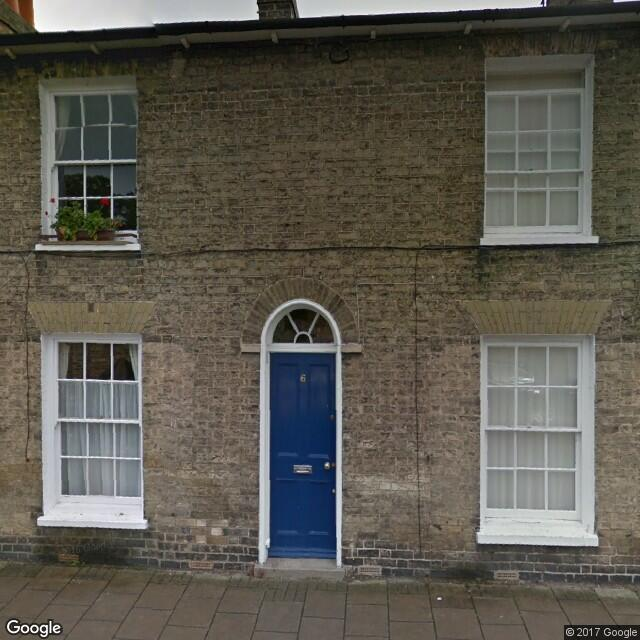
\includegraphics[width=45px]{images//0001000010058205_KqBBtZS8ecncUe8oqjErqQ.jpg} & 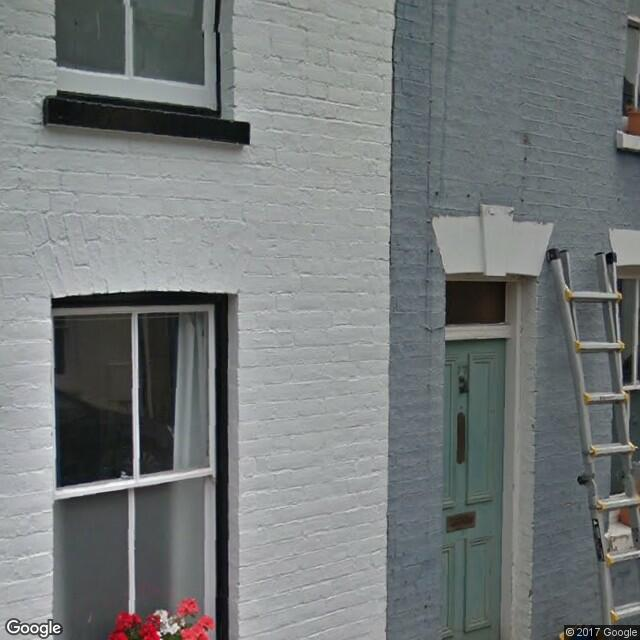
\includegraphics[width=45px]{images//0001000010102767_u_7T3iAyG9xNgeN_ETY7aQ.jpg} & 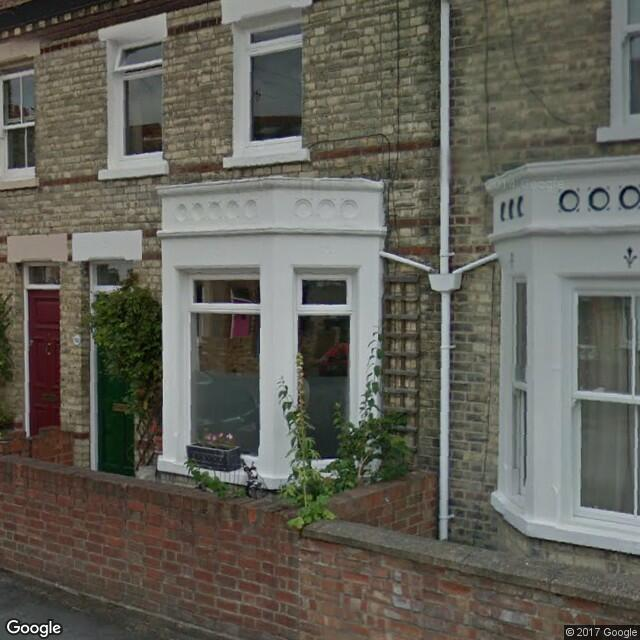
\includegraphics[width=45px]{images//0001000010141478_FT9houQ2x66NPnNEGxTkvA.jpg} & 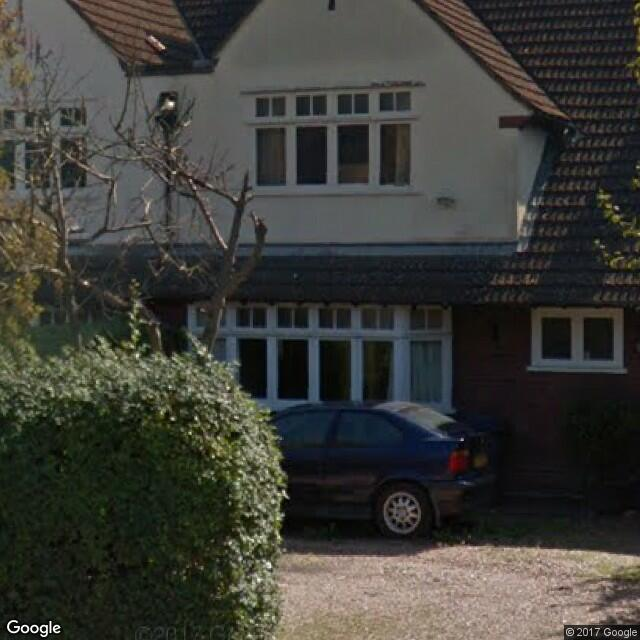
\includegraphics[width=45px]{images//0001000010065714_pzExlR026vDKdQaJiLkdkw.jpg} & 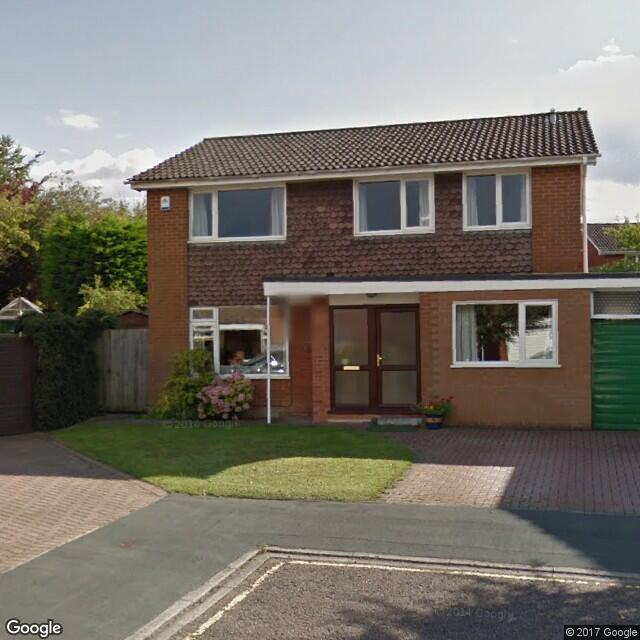
\includegraphics[width=45px]{images//0001000010137600_qYxYCsLRPpOfCyv8IjfnlA.jpg} & 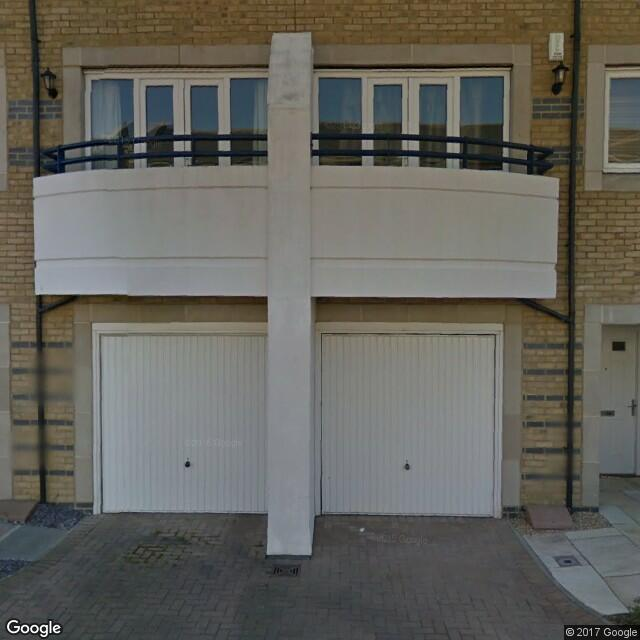
\includegraphics[width=45px]{images//1000002057677225_srJnz_31ujVFzn-xh_DYfw.jpg} & 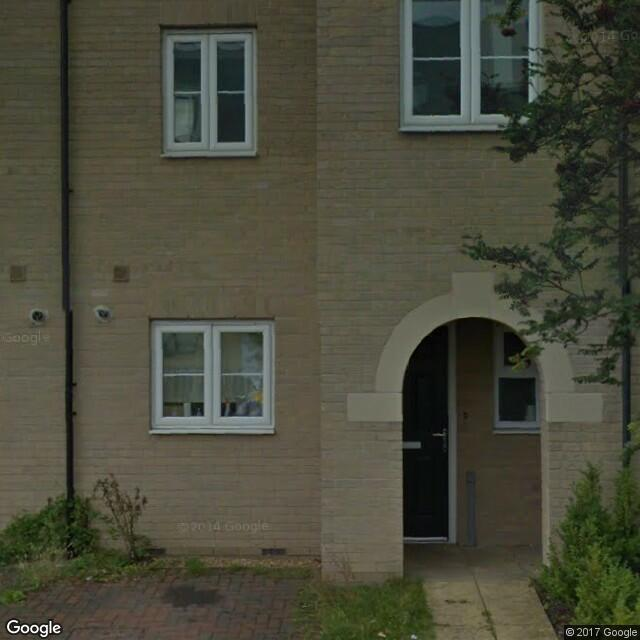
\includegraphics[width=45px]{images//1000002500413689_VylY6Sy3vLvjqbtHeryMdQ.jpg} \\ 
  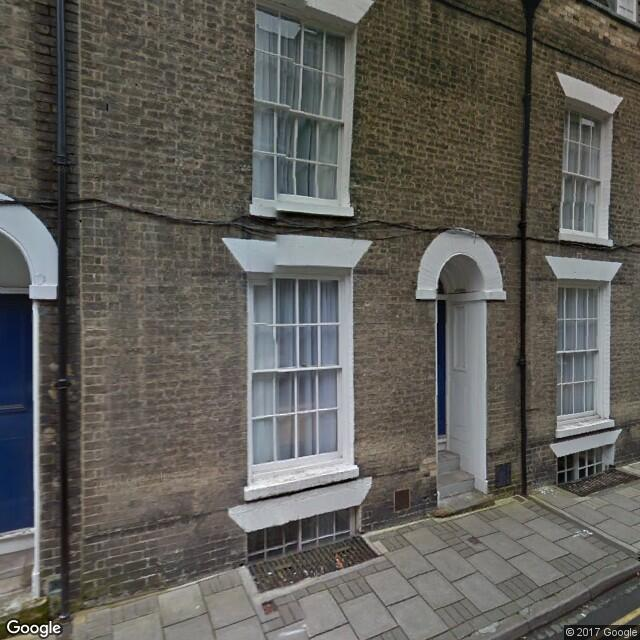
\includegraphics[width=45px]{images//0001000010056385_XQsTJ2p5Te54CScFmblMHA.jpg} & 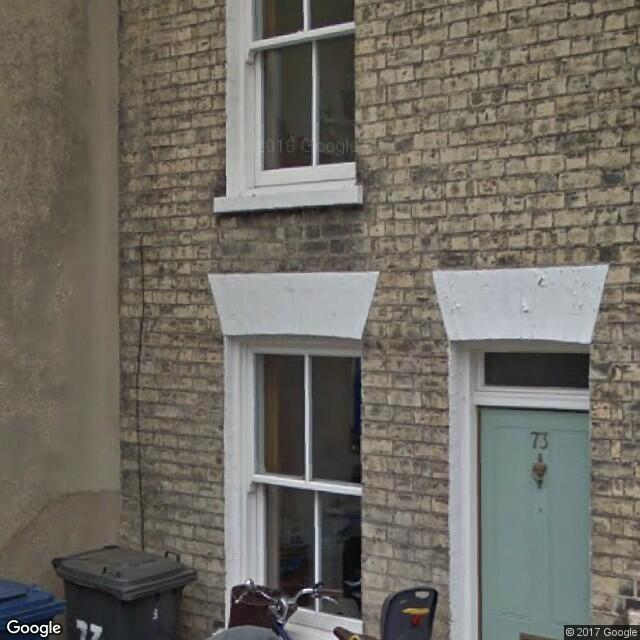
\includegraphics[width=45px]{images//0001000010102769_c_e4WlmafqN2JXQ2ZhYEkw.jpg} & 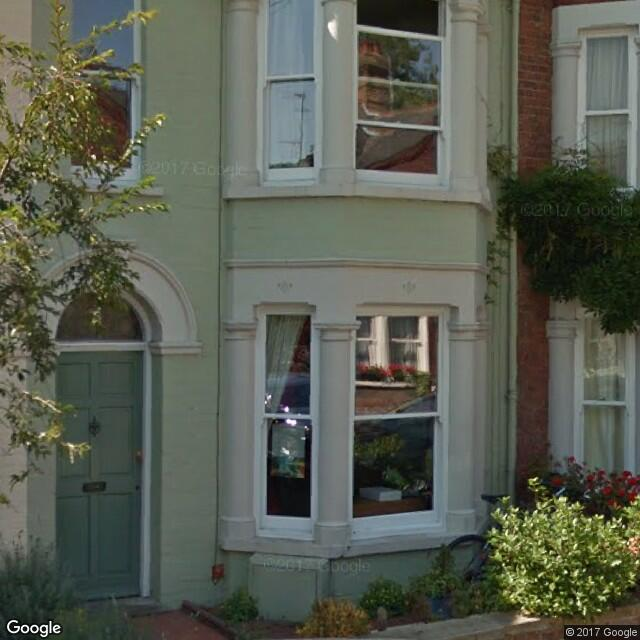
\includegraphics[width=45px]{images//0001000010017237_yWs7fxQ0r8Ecx_ajaYc-rg.jpg} & 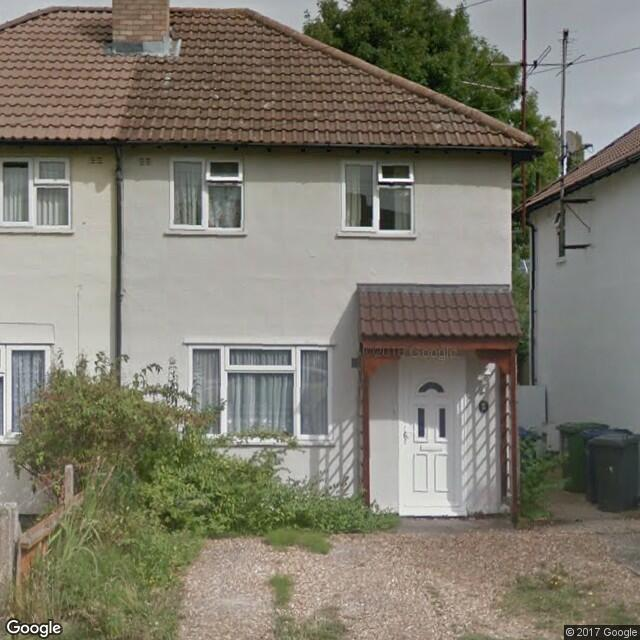
\includegraphics[width=45px]{images//0001000010141115_xG0eSas79cN59fH4xvm5Yw.jpg} & 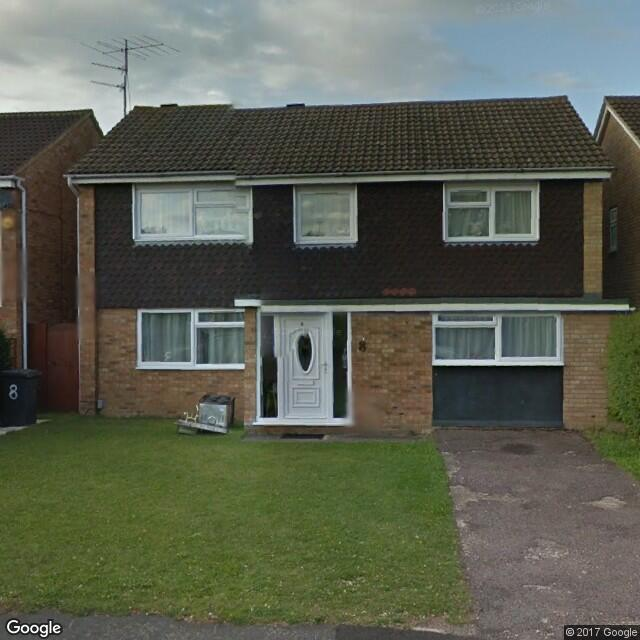
\includegraphics[width=45px]{images//0001000010023665_B2Is2WMV8SGjf7Tg9tLS7w.jpg} & 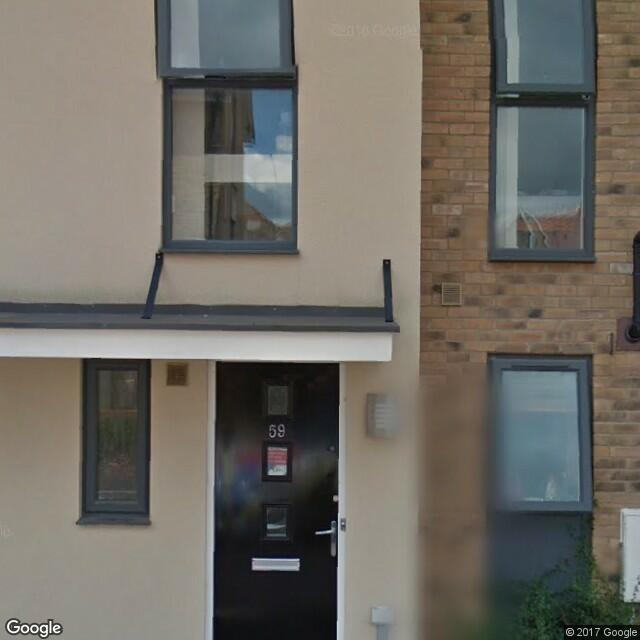
\includegraphics[width=45px]{images//1000002500748070_DkW5iwQYtGox02-tF2i9rQ.jpg} & 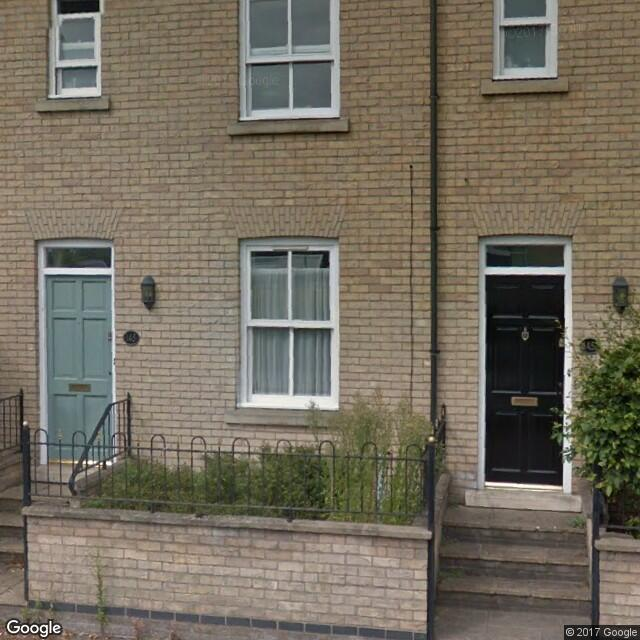
\includegraphics[width=45px]{images//0001000010176986_bNOie2HS7GPQxPOtoevEHw.jpg} \\ 
  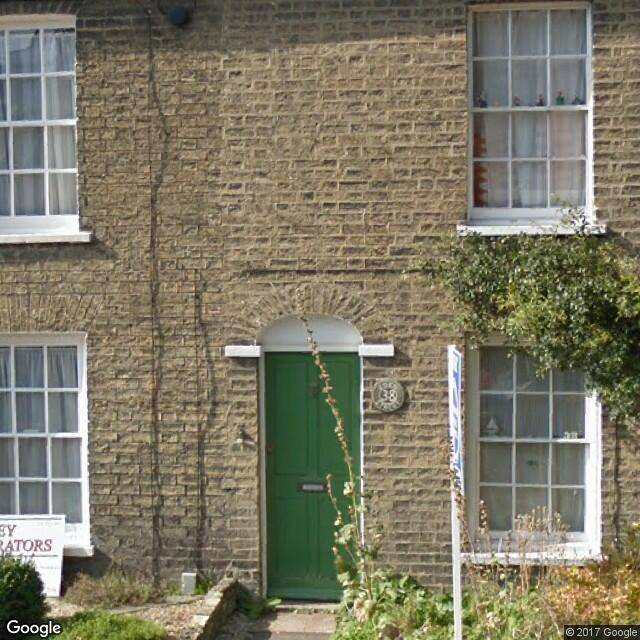
\includegraphics[width=45px]{images//0001000010058145_xBAz4f8lI2MTivvvWv6wyQ.jpg} & 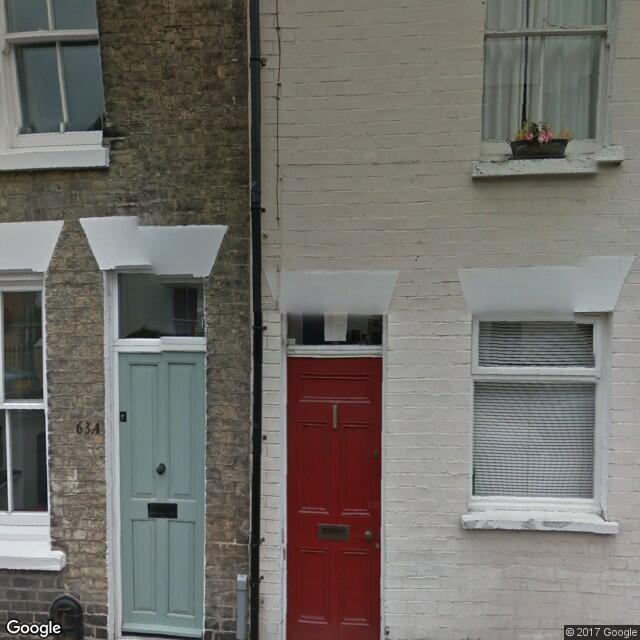
\includegraphics[width=45px]{images//0001000010103488_Y1L2niOkEGB1IKe4tsl1yw.jpg} & 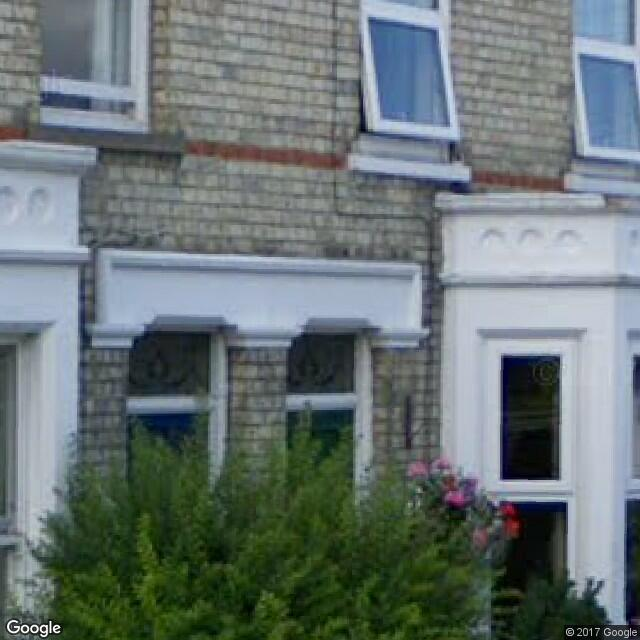
\includegraphics[width=45px]{images//0001000010021367_JF-P4lOQQouZ6lHtM4J3oA.jpg} & 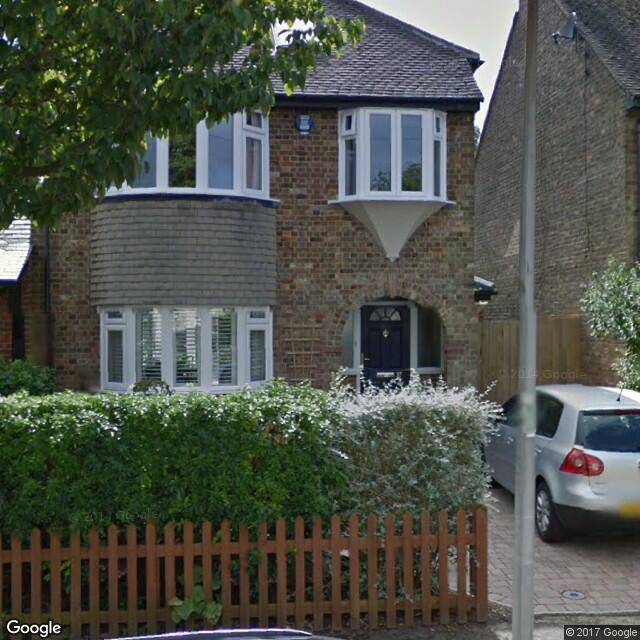
\includegraphics[width=45px]{images//0001000010065349_HDvoqsiHXGx4xc62JSUNJA.jpg} & 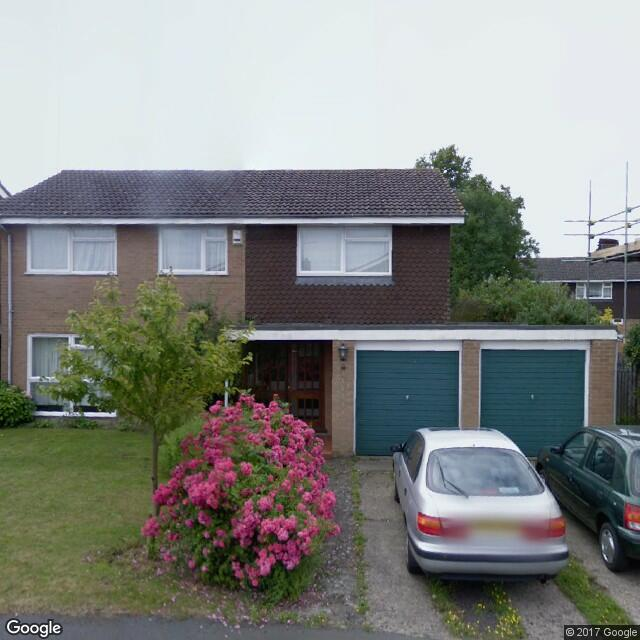
\includegraphics[width=45px]{images//0001000009993819_748OTBKSFyJZU2DP7TbboQ.jpg} & 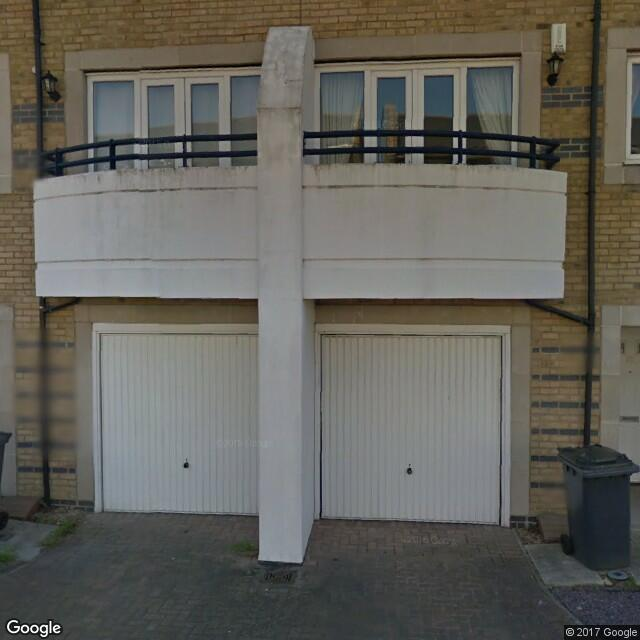
\includegraphics[width=45px]{images//1000002057677000_8l6ywNIej2136uZeb3qKqA.jpg} & 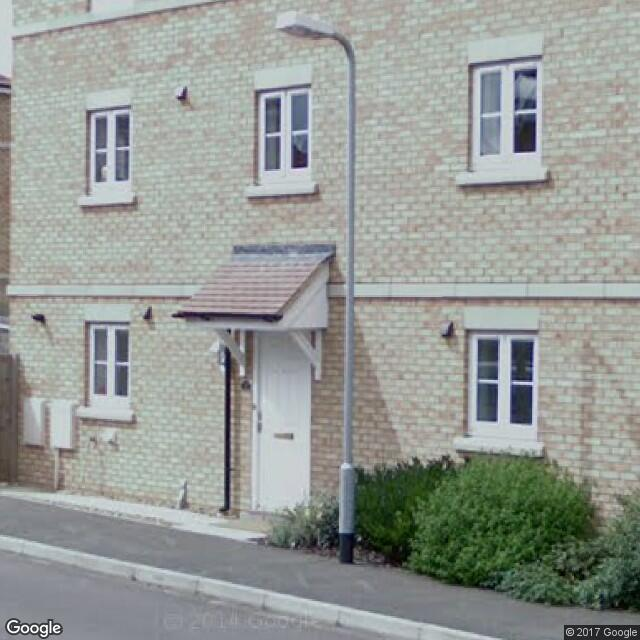
\includegraphics[width=45px]{images//1000002500088807_4vu-eMLHmhX3JmHNwyulmQ.jpg} \\ 
  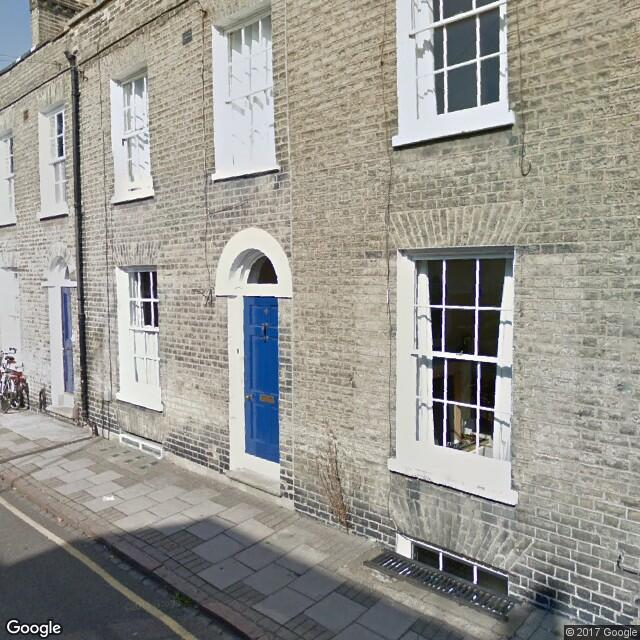
\includegraphics[width=45px]{images//0001000010059206__nUymOPxCgpQugahoE7EPw.jpg} & 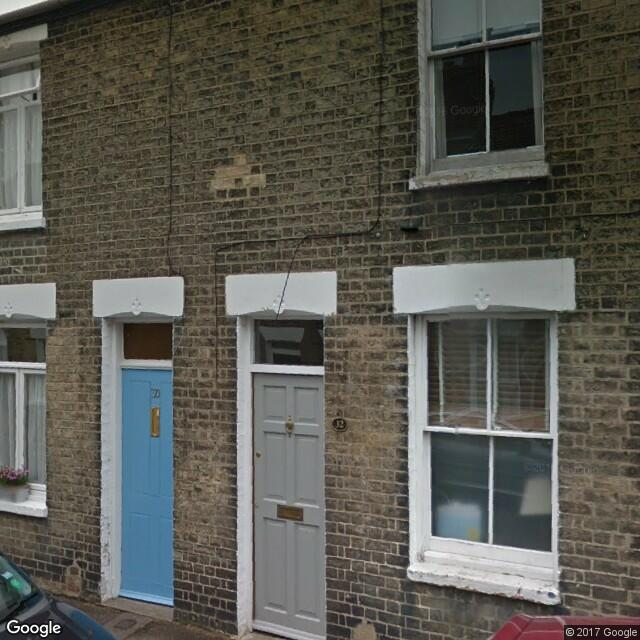
\includegraphics[width=45px]{images//0001000010103870_ywN_BuvuLW6kbLLP0QgJMA.jpg} & 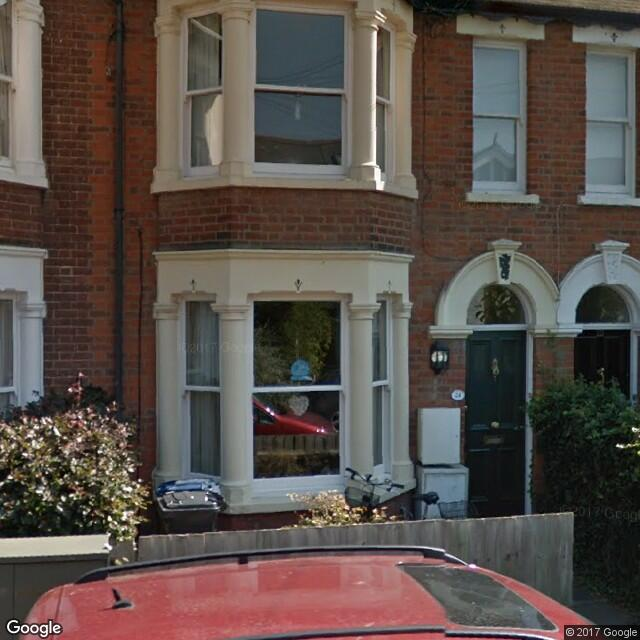
\includegraphics[width=45px]{images//0001000010017412_aOsldmaOT-MAce6q6qkmTQ.jpg} & 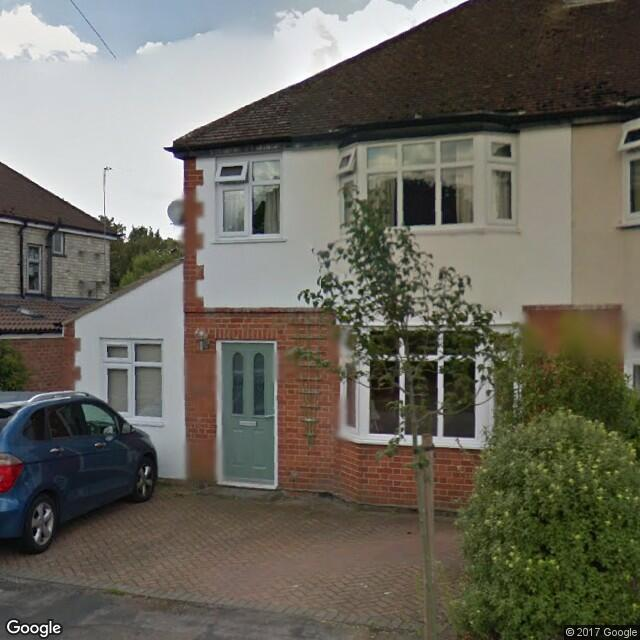
\includegraphics[width=45px]{images//0001000010107971_veilqmDOA-AfCuz4tWyg7g.jpg} & 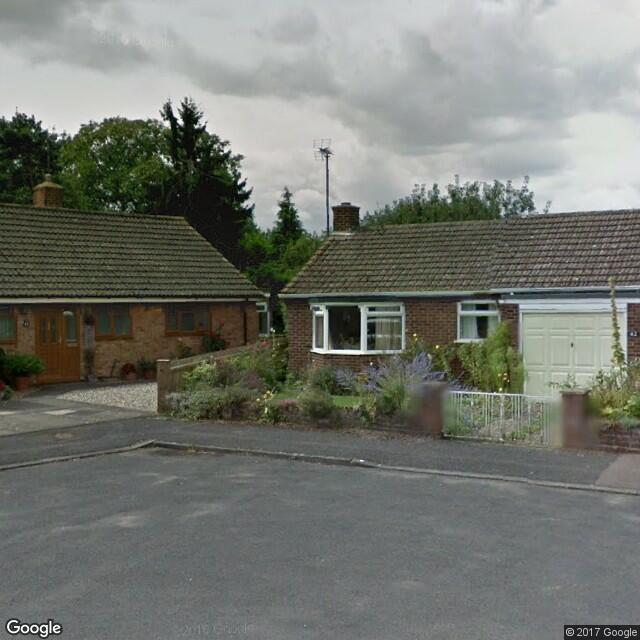
\includegraphics[width=45px]{images//0001000010025542_8rvXwCYBTCQu0eVM9nhN9Q.jpg} & 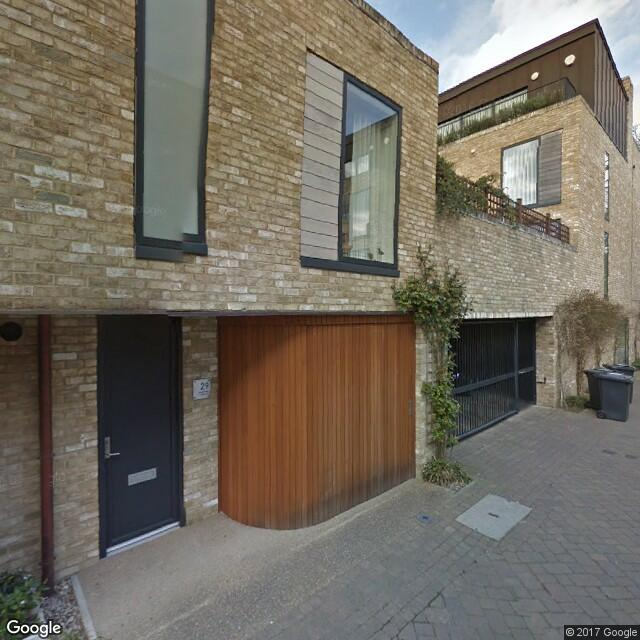
\includegraphics[width=45px]{images//1000002500555322_FffLx_XVBUOvZgiXRdSAnA.jpg} & 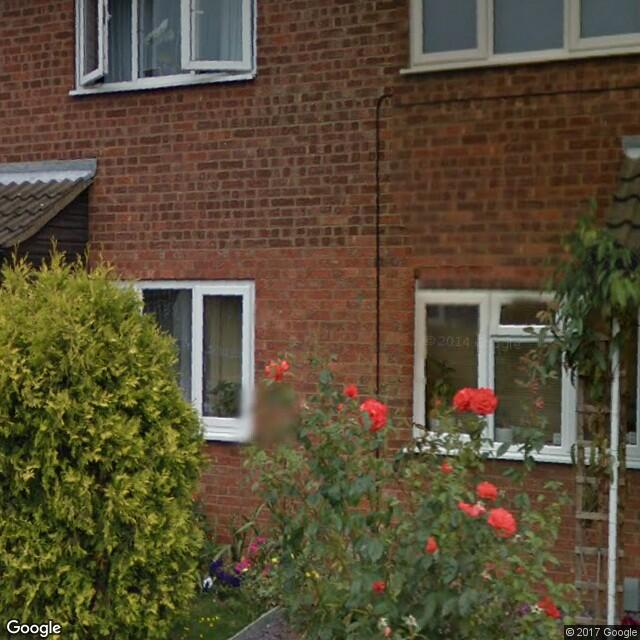
\includegraphics[width=45px]{images//0001000010066754_dJmIRHcgebzrGzDR_Cahaw.jpg} \\ 
  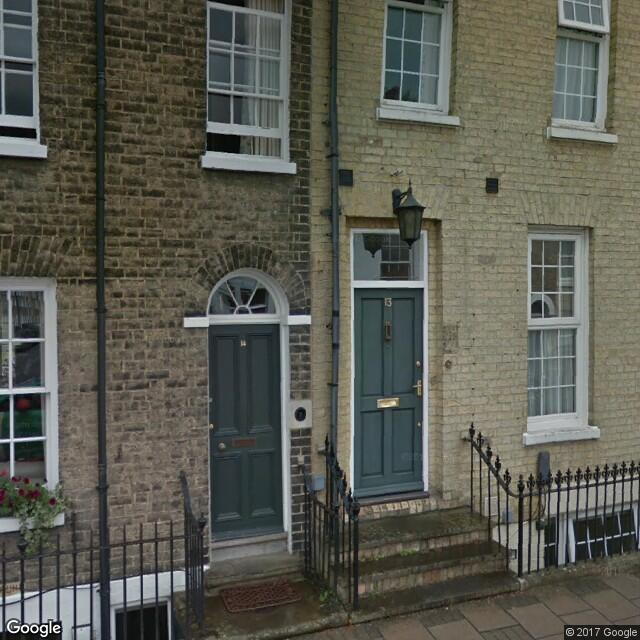
\includegraphics[width=45px]{images//0001000010060140_8_DVq9QCmlMezNuDHGixwg.jpg} & 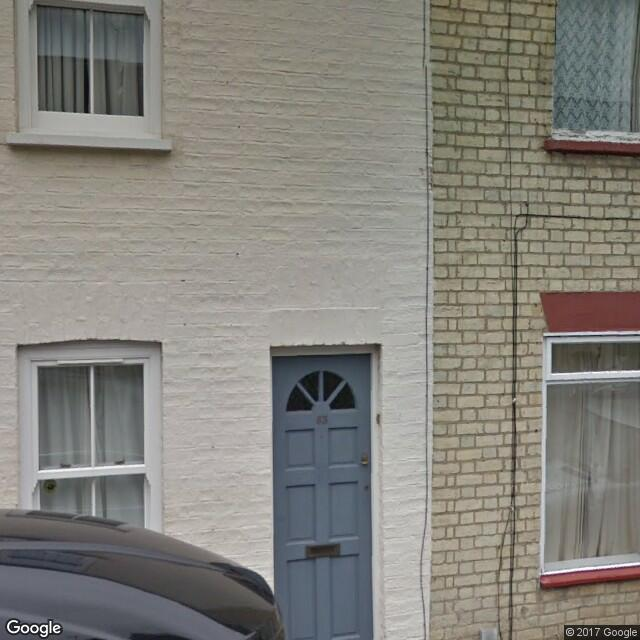
\includegraphics[width=45px]{images//0001000010103819_mF6OqQrRTOlAoGdaraQsTQ.jpg} & 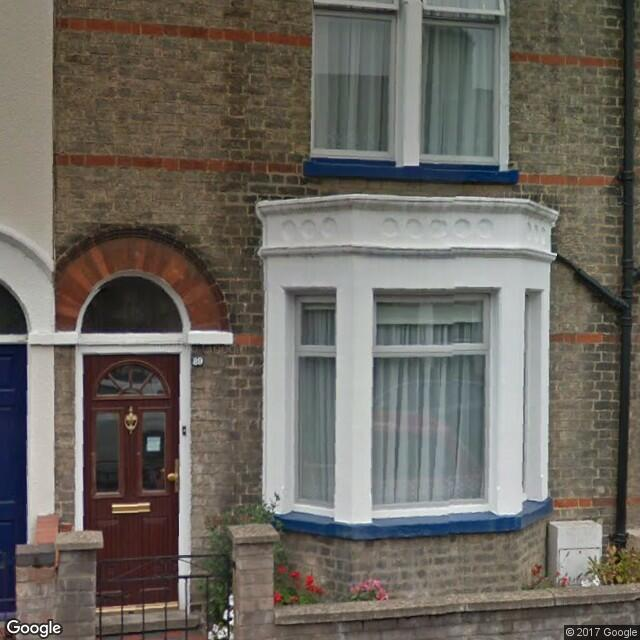
\includegraphics[width=45px]{images//0001000010097999_xTD3YceIrtPJZwPz5d0G6Q.jpg} & 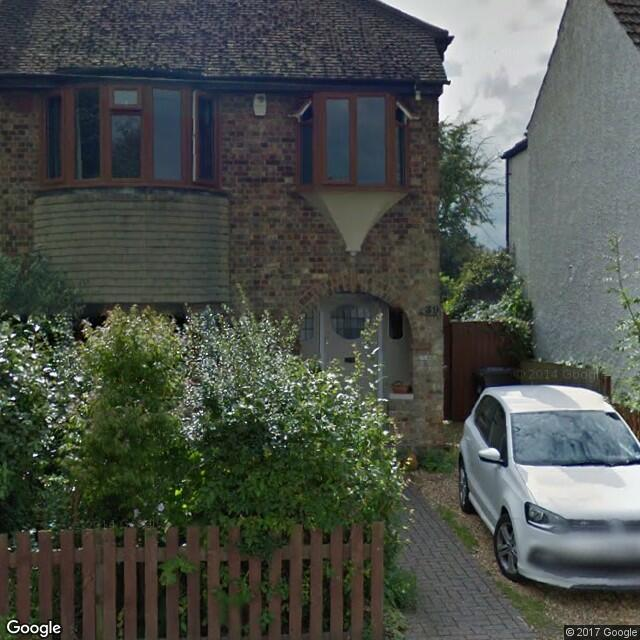
\includegraphics[width=45px]{images//0001000010065347_pouLRqJd7pkk41jryvYQ4A.jpg} & 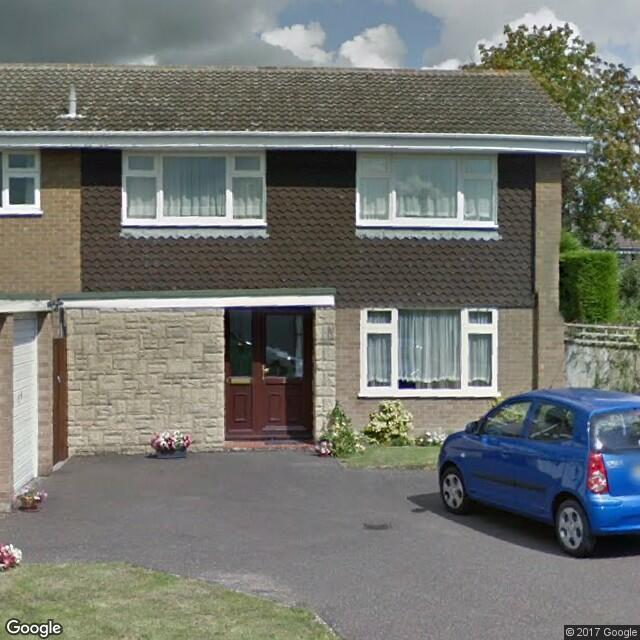
\includegraphics[width=45px]{images//0001000009992776_QxMV8eRavS1riXfGzpSkBw.jpg} & 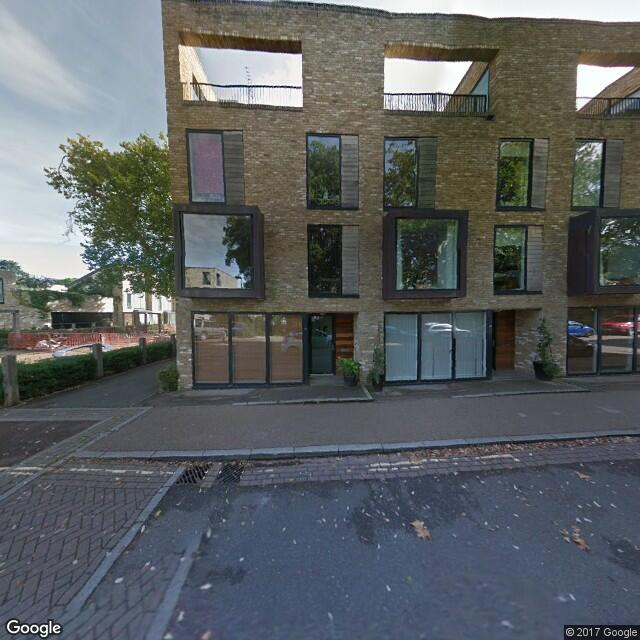
\includegraphics[width=45px]{images//1000002500555341_NVXmLF7mim1nGBZAdgw_ew.jpg} & 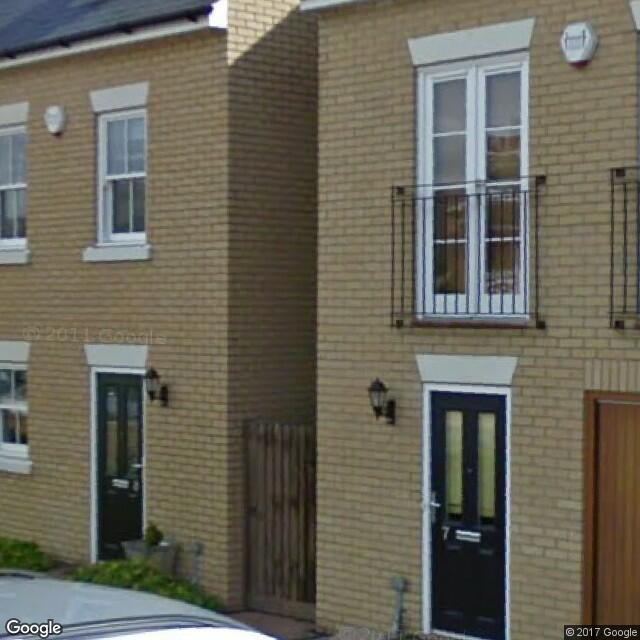
\includegraphics[width=45px]{images//1000002500569086_g5RwBQ7D5edS2obfSogNIw.jpg} \\ 
  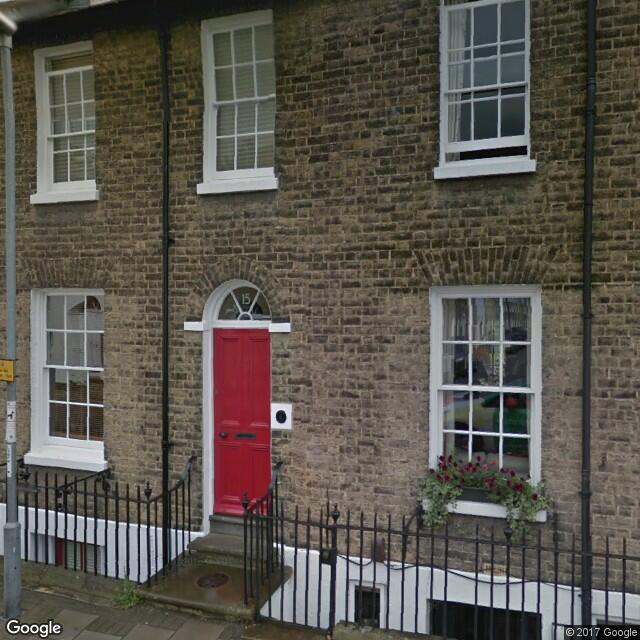
\includegraphics[width=45px]{images//0001000010060139_8_DVq9QCmlMezNuDHGixwg.jpg} & 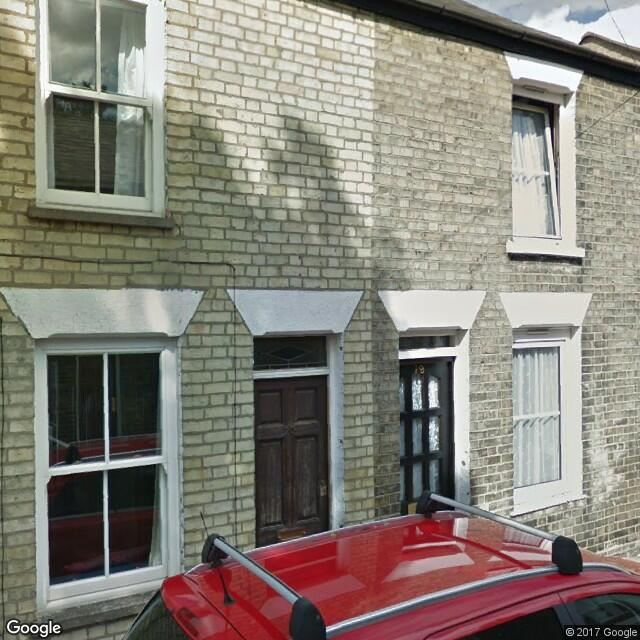
\includegraphics[width=45px]{images//0001000010101711_wNQ403N-0pQd5fChNztfYA.jpg} & 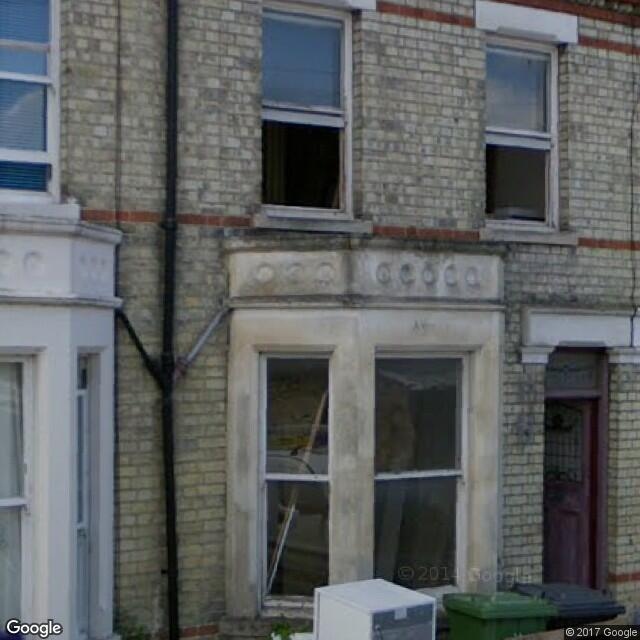
\includegraphics[width=45px]{images//0001000010021374_55tKverBLF4C0oo8U4XABg.jpg} & 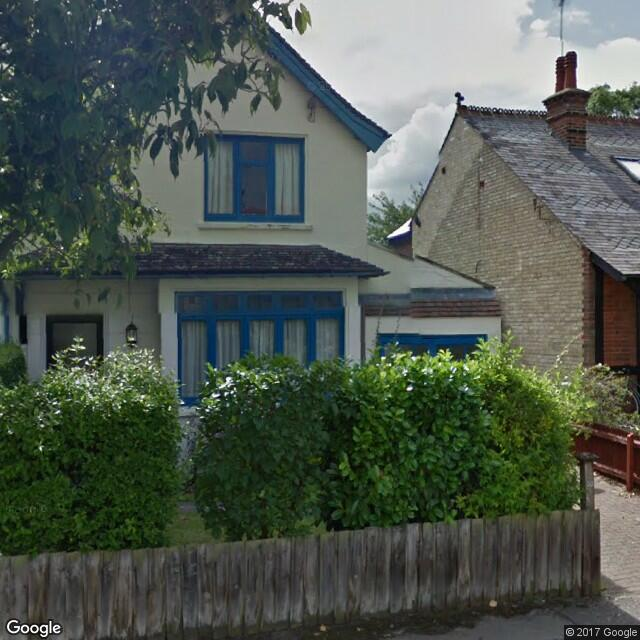
\includegraphics[width=45px]{images//0001000010065352_kDKqKaGpPwLeCBKJIQmeCg.jpg} & 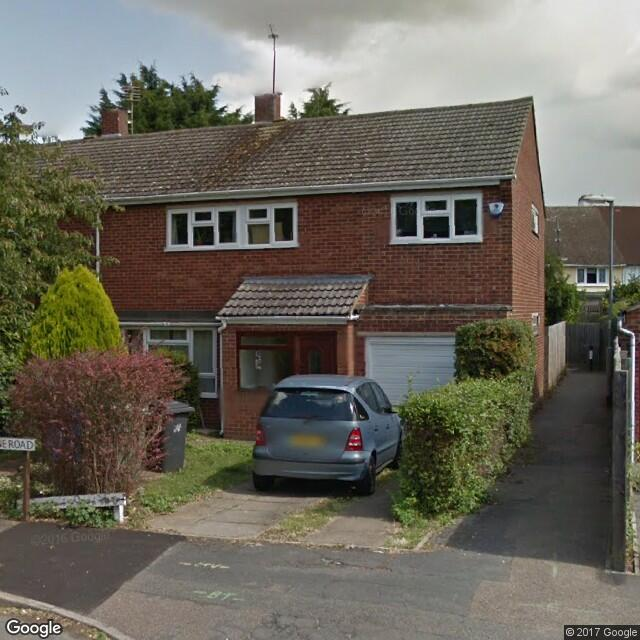
\includegraphics[width=45px]{images//0001000010015484_zlR1vVJ7F0L6hcsFoZEydw.jpg} & 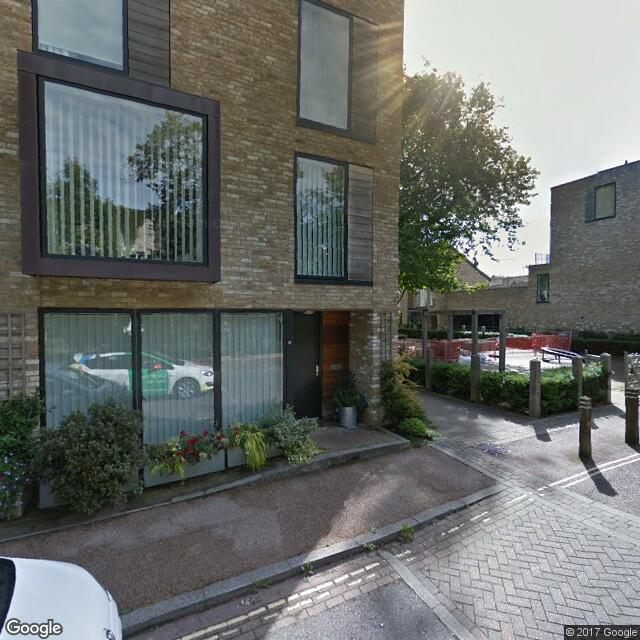
\includegraphics[width=45px]{images//1000002500548748_i6QAKtN2HhGsTVDBan2DKw.jpg} & 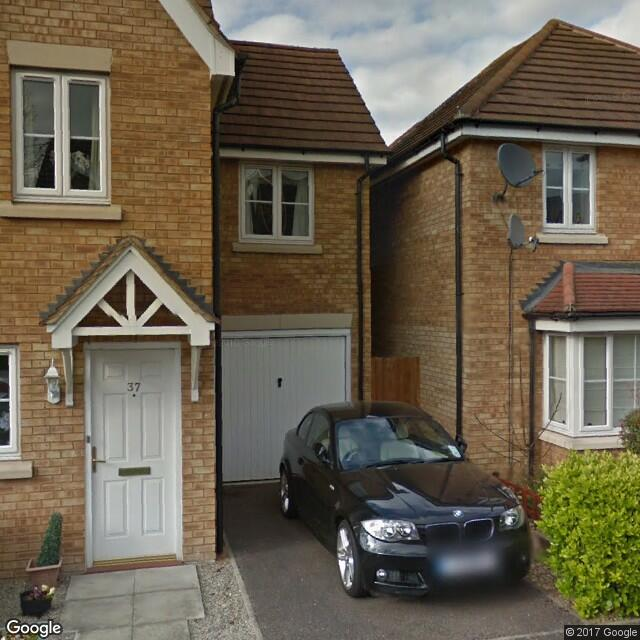
\includegraphics[width=45px]{images//1000002057955271_dMXMWNaIwddWdHidEuXowA.jpg} \\ 
  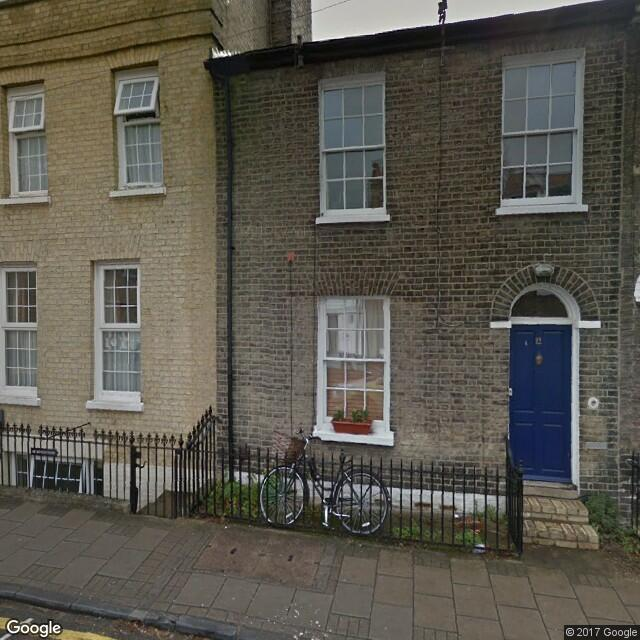
\includegraphics[width=45px]{images//0001000010060141_W3ZIE8mPY6LJb-_hKatlUw.jpg} & 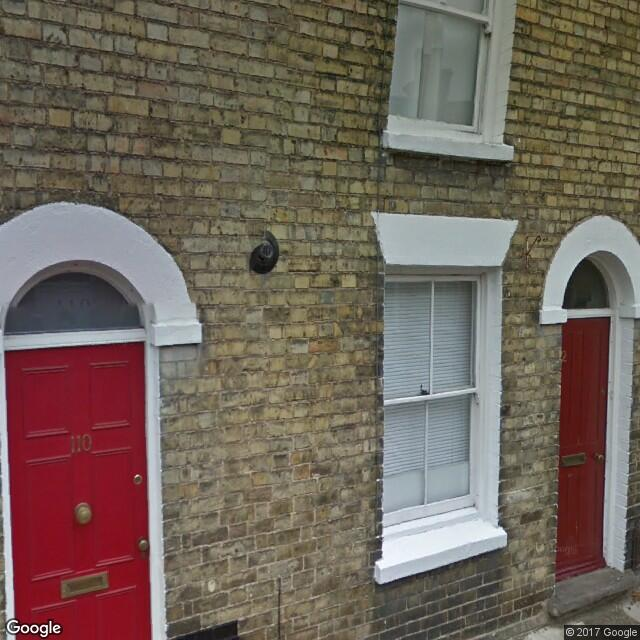
\includegraphics[width=45px]{images//0001000010103226_XO6qx_5Q9tNnNF958OBO3g.jpg} & 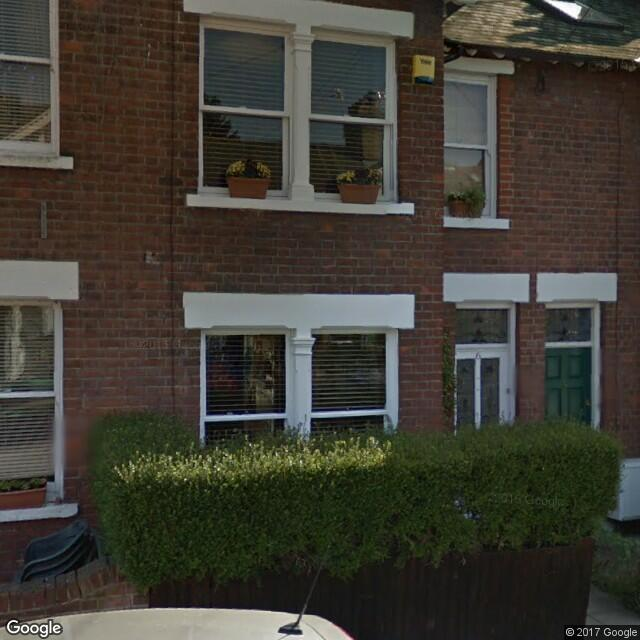
\includegraphics[width=45px]{images//0001000010017109_MbGvl1GxhZjQ_qhD7puDBw.jpg} & 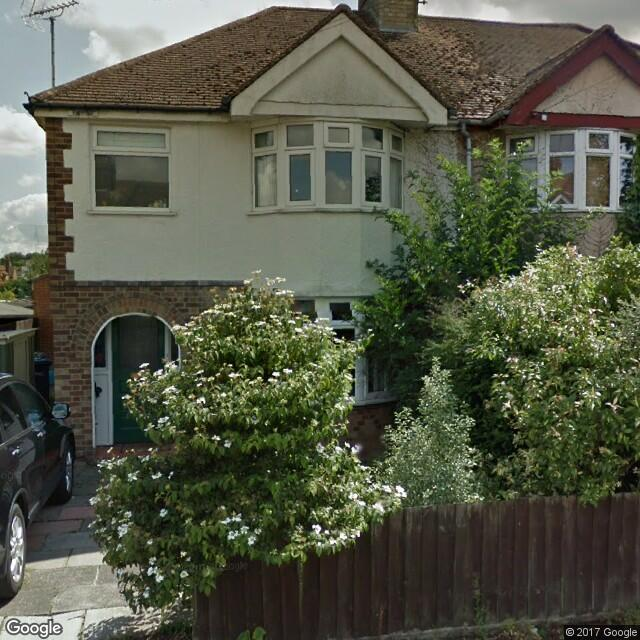
\includegraphics[width=45px]{images//0001000009995496_N4NgCofyWASyYfcSPTjdBA.jpg} & 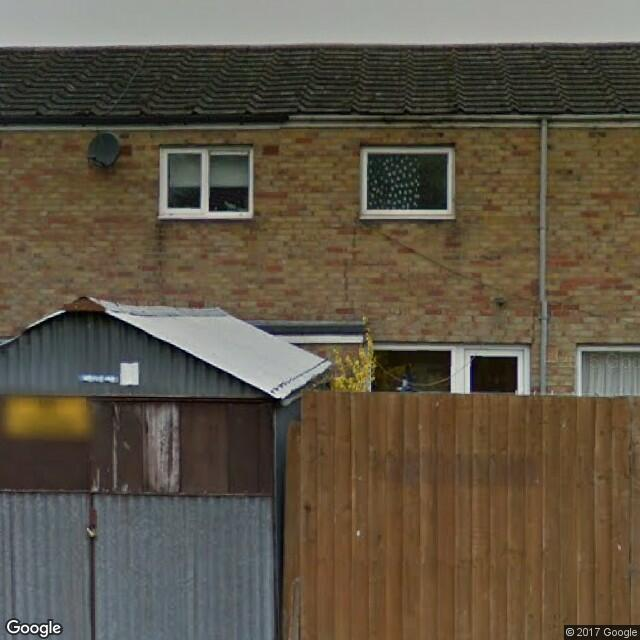
\includegraphics[width=45px]{images//0001000010068890_aswyTpwrE_IfdbINnYx7XQ.jpg} & 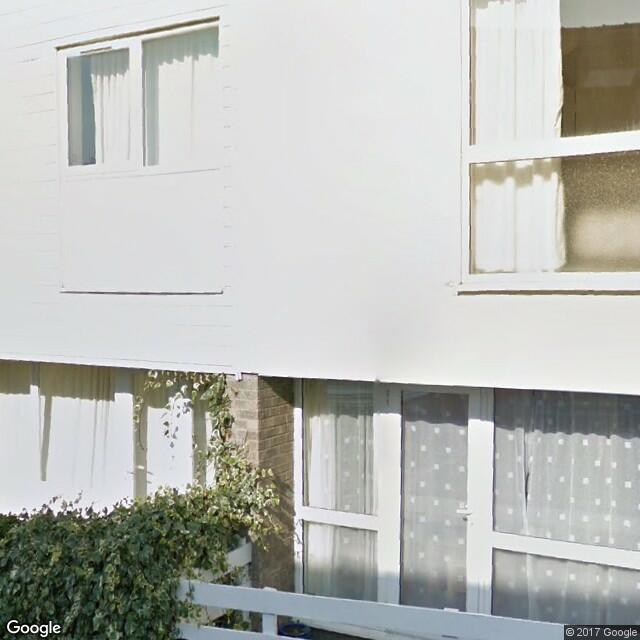
\includegraphics[width=45px]{images//0001000010104229_qFV1-weLxn8SRW4Ib2wexQ.jpg} & 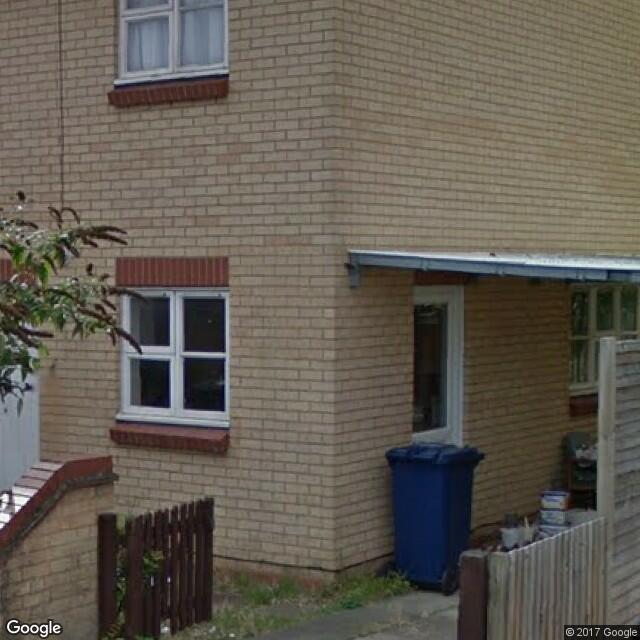
\includegraphics[width=45px]{images//0001000010199676_smIagQ34MLIcJOrjvIu9uw.jpg} \\ 
  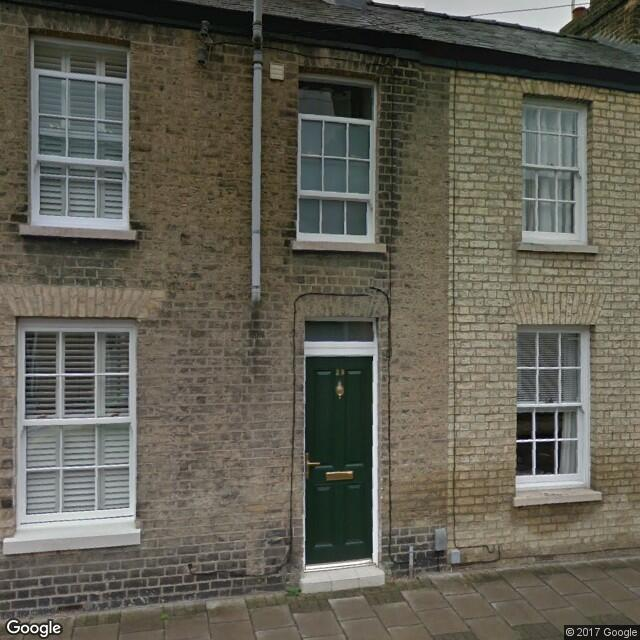
\includegraphics[width=45px]{images//0001000010059966_e8c8bmHUpyKpiIZ1YO9ypg.jpg} & \includegraphics[width=45px]{images//0001000010101704_ZQFxujswdAj7EGqRlp8sXQ.jpg} & \includegraphics[width=45px]{images//0001000010017361_WxMCM3nht5EX_K9pqIK-kQ.jpg} & \includegraphics[width=45px]{images//0001000010066620_4TqmJVLf3urSJo4ESg1zfw.jpg} & \includegraphics[width=45px]{images//0001000010023689_KpXUKEdjoQ9swgoB2oXA3w.jpg} & \includegraphics[width=45px]{images//1000002500748058_DkW5iwQYtGox02-tF2i9rQ.jpg} & \includegraphics[width=45px]{images//0001000010066718_dJmIRHcgebzrGzDR_Cahaw.jpg} \\ 
  \includegraphics[width=45px]{images//0001000010060813_VlKeIvrTv6UwOE9HD2LgJg.jpg} & \includegraphics[width=45px]{images//0001000010103859_P5YwPMree6QCxExkKqIzbw.jpg} & \includegraphics[width=45px]{images//0001000010141515_5g5Bhsn_4iW-90aFMrIaSA.jpg} & \includegraphics[width=45px]{images//0001000010066361_gliMrVbagcfkfZjLw4mKlw.jpg} & \includegraphics[width=45px]{images//1000002500527045_p4zTtg8OzsbWjHYscCf-rA.jpg} & \includegraphics[width=45px]{images//1000002500748076_zDr74LLmVeyKyx7dPnXK6A.jpg} & \includegraphics[width=45px]{images//1000002500413682_drSMg0SQ9TU4Og8pXOgSxw.jpg} \\ 
  \includegraphics[width=45px]{images//0001000010059967_e8c8bmHUpyKpiIZ1YO9ypg.jpg} & \includegraphics[width=45px]{images//0001000010103388_CZH157SXYmF3dEVMKlWBfQ.jpg} & \includegraphics[width=45px]{images//0001000010025644_bJ8zv37pDsP0CImvDMKC0w.jpg} & \includegraphics[width=45px]{images//0001000010144910_COpJNwPw67J78VXCoN_HMA.jpg} & \includegraphics[width=45px]{images//0001000009992797_JUTa4GsWaXplyCP6XeVAvw.jpg} & \includegraphics[width=45px]{images//1000002500086356_n92s3snPX2zAwEiJnA-Pxg.jpg} & \includegraphics[width=45px]{images//0001000010176201_dDyXoyEbeMXUhCagwazbiA.jpg} \\ 
   \hline
\end{tabular}
\label{fig:vint_examples}
\begin{minipage}{0.75\textwidth}
\footnotesize \emph{Notes:} In these images, it is clear that much of the visual heterogeneity in style is due to differences in windows, doors, and rooflines. For example, there are clear differences across styles based on groupings and number of panes per windows and shapes of pediments, lintels, or fanlights above doors. Some characteristics stand out such as the presence of bay windows for Late V./Edwardian properties and angularity, asymmetry of windows in the Contemporary class, and roofing style and setback in the Postwar period.
\end{minipage}
\end{figure}

\clearpage

\begin{figure}[hbt]
  \caption{Improving Camera Aim for Automatic Image Collections}
  \centering
  \vspace{0.25cm}
  \begin{tabular}{cc}
    \includegraphics[width=0.55\textwidth]{figures/84VineryRD.png} & \includegraphics[width=0.3\textwidth]{figures/84VineryRoadGoodAim.png} \\
    \emph{(a) Default Camera Aim} & \emph{(b) Improved Aim}\\

\end{tabular}

  \label{fig:84Vin}
\begin{minipage}{0.8\textwidth}
\footnotesize 
\vspace{0.25cm}
\emph{Notes:} For the UK, the Google Street View API returns the coordinates of the nearest camera snapshot for a given location but fails to provide an accurate orientation and zoom-level of the camera needed to capture the front of the building exactly. In (a) the building of interest is not even visible in the picture. The image at (b) was taken with pan and zoom parameters, derived by our viewshed algorithm. Even for a terraced property, the structure contains minimal neighbor information, the roofline is captured, vehicles on the street are not visible the image is not obstructed by other structures.  
\emph{Image source}: Google Street View. 
\end{minipage}
\end{figure}

\begin{figure}[hbt]
  \caption{Image Collection on Google Street View: Camera Direction and Zoom}
  \centering
    \includegraphics[width=0.8\textwidth]{figures/fan.png}
  \label{fig:fan}
\begin{minipage}{0.8\textwidth}
\vspace{0.25cm}
\footnotesize \emph{Notes:} We first look up the nearest Google Street View panorama point (green dot) based on the centroid (red dot) coordinates of a given building obtained from Ordnance Survey maps. A viewshed analysis identifies which exterior walls are visible from the panorama point, ignoring any wall segments where the direct line of sight from the panorama point is obstructed by other buildings. The camera bearing (green line) and zoom factor are based on the angle of the most outer lines of sight (blue lines).
\end{minipage}
\end{figure}

\newpage





\begin{table}[!htb]
	\caption{Confusion matrix for classification based on images of property and its nearest neighbor}
	\label{tab:confmat}
	\centering
\begingroup\footnotesize
	\emph{}
\begin{tabular}{lrrrrrrr}
	& \multicolumn{7}{c}{\rule{0pt}{4ex}    \emph{Panel A: Model based on individual building and nearest neighbor} \rule{0pt}{4ex}    }\\
	\toprule
	\emph{Machine} & \multicolumn{7}{c}{\emph{Architects}} \\
	\cmidrule(lr){2-8}
	& Georgian & Early Vic. & Late V./Edw. & Interwar & Postwar & Cont. & Revival \\
  \cmidrule(lr){1-1}
\cmidrule(lr){2-8}
	Georgian & 284 & 109 & 77 & 38 & 14 & 23 & 22 \\
	  Early Vic. & 50 & 1755 & 427 & 86 & 86 & 56 & 34 \\
	  Late V./Edw. & 10 & 172 & 3260 & 213 & 56 & 21 & 29 \\
	  Interwar & 10 & 46 & 254 & 5884 & 997 & 56 & 54 \\
	  Postwar & 1 & 17 & 48 & 514 & 3914 & 74 & 40 \\
	  Cont. & 3 & 50 & 63 & 101 & 333 & 855 & 69 \\
	  Revival & 3 & 29 & 45 & 139 & 145 & 98 & 501 \\
		\cmidrule(lr){1-1}
\cmidrule(lr){2-8}
	  Georgian & 79\% & 5\% & 2\% & 1\% & 0\% & 2\% & 3\% \\
	  Early Vic. & 14\% & 81\% & 10\% & 1\% & 2\% & 5\% & 5\% \\
	  Late V./Edw. & 3\% & 8\% & 78\% & 3\% & 1\% & 2\% & 4\% \\
	  Interwar & 3\% & 2\% & 6\% & 84\% & 18\% & 5\% & 7\% \\
	  Postwar & 0\% & 1\% & 1\% & 7\% & 71\% & 6\% & 5\% \\
	  Cont. & 1\% & 2\% & 2\% & 1\% & 6\% & 72\% & 9\% \\
	  Revival & 1\% & 1\% & 1\% & 2\% & 3\% & 8\% & 67\% \\
		\cmidrule(lr){1-1}
\cmidrule(lr){2-8}
	  Recall & 0.79 & 0.81 & 0.78 & 0.84 & 0.71 & 0.72 & 0.67 \\
	  Precision & 0.50 & 0.70 & 0.87 & 0.81 & 0.85 & 0.58 & 0.52 \\
	  $F_1$-score & 0.61 & 0.75 & 0.82 & 0.82 & 0.77 & 0.64 & 0.59 \\

		\cmidrule(lr){1-1} \cmidrule(lr){2-8}
		& \multicolumn{7}{c}{ \emph{ Panel B: Model based on individual building and nearest neighbor, high confidence only} \rule{0pt}{4ex}    }\\
		\cmidrule(lr){1-1} \cmidrule(lr){2-8}

Georgian & 122 & 31 & 9 & 4 & 2 & 1 & 5 \\
Early Vic. & 30 & 1,926 & 324 & 19 & 40 & 15 & 7 \\
  Late V./Edw. & 0 & 105 & 2,941 & 68 & 19 & 0 & 9 \\
 Interwar & 6 & 6 & 81 & 3,230 & 369 & 10 & 14 \\
 Postwar & 0 & 3 & 5 & 96 & 1,831 & 9 & 6 \\
 Cont. & 0 & 8 & 7 & 4 & 33 & 236 & 18 \\
 Revival & 3 & 2 & 0 & 14 & 10 & 4 & 154 \\
 \cmidrule(lr){1-1}
\cmidrule(lr){2-8}
 Georgian & 76\% & 2\% & 0\% & 0\% & 0\% & 0\% & 2\% \\
 Early Vic. & 19\% & 93\% & 10\% & 1\% & 2\% & 6\% & 3\% \\
  Late V./Edw. & 0\% & 5\% & 87\% & 2\% & 1\% & 0\% & 4\% \\
 Interwar & 4\% & 0\% & 2\% & 94\% & 16\% & 4\% & 7\% \\
 Postwar & 0\% & 0\% & 0\% & 3\% & 80\% & 3\% & 3\% \\
 Cont. & 0\% & 0\% & 0\% & 0\% & 1\% & 86\% & 9\% \\
Revival & 2\% & 0\% & 0\% & 0\% & 0\% & 2\% & 72\% \\
\cmidrule(lr){1-1}
\cmidrule(lr){2-8}
Recall & 0.76 & 0.93 & 0.87 & 0.94 & 0.79 & 0.86 & 0.72 \\
 Precision & 0.70 & 0.82 & 0.94 & 0.87 & 0.94 & 0.77 & 0.82 \\
$F_1$-score & 0.73 & 0.87 & 0.90 & 0.90 & 0.86 & 0.81 & 0.77 \\

\cmidrule(lr){1-1} \cmidrule(lr){2-8}
& \multicolumn{7}{c}{ \emph{Panel C: Model based on individual buildings only} \rule{0pt}{4ex}    }\\
\cmidrule(lr){1-1} \cmidrule(lr){2-8}

	Georgian & 267 & 121 & 110 & 46 & 33 & 36 & 17 \\
	  Early.Vic. & 50 & 1673 & 438 & 112 & 107 & 63 & 52 \\
	  Late V./Edw. & 19 & 183 & 3099 & 272 & 86 & 33 & 44 \\
	  Interwar & 12 & 71 & 335 & 5786 & 1419 & 84 & 82 \\
	  Postwar & 2 & 24 & 56 & 462 & 3364 & 75 & 38 \\
	  Cont. & 5 & 63 & 82 & 141 & 366 & 778 & 79 \\
	  Revival & 6 & 43 & 54 & 156 & 170 & 114 & 437 \\
	\cmidrule(lr){1-1}
\cmidrule(lr){2-8}
	  Georgian & 74\% & 6\% & 3\% & 1\% & 1\% & 3\% & 2\% \\
	  Early.Vic. & 14\% & 77\% & 10\% & 2\% & 2\% & 5\% & 7\% \\
	  Late V./Edw. & 5\% & 8\% & 74\% & 4\% & 2\% & 3\% & 6\% \\
	  Interwar & 3\% & 3\% & 8\% & 83\% & 26\% & 7\% & 11\% \\
	  Postwar & 1\% & 1\% & 1\% & 7\% & 61\% & 6\% & 5\% \\
	  Cont. & 1\% & 3\% & 2\% & 2\% & 7\% & 66\% & 11\% \\
	  Revival & 2\% & 2\% & 1\% & 2\% & 3\% & 10\% & 58\% \\
		\cmidrule(lr){1-1}
\cmidrule(lr){2-8}
	  Recall & 0.74 & 0.77 & 0.74 & 0.83 & 0.61 & 0.66 & 0.58 \\
	  Precision & 0.42 & 0.67 & 0.83 & 0.74 & 0.84 & 0.51 & 0.45 \\
	  $F_1$-score & 0.54 & 0.72 & 0.78 & 0.78 & 0.70 & 0.58 & 0.51 \\
	 \bottomrule
\end{tabular}

\begin{minipage}{\textwidth}
\footnotesize
\vspace{0.25cm}
	\emph{Notes:} Cross-tabulation of out-of-sample predictions by the machine versus the architects' classification.
	\emph{Recall} is the share of buildings from an architects' category being predicted correctly (diagonal in mid panel) and \emph{Precision} is the share of buildings predicted to belong to a category that are indeed from that category.
	$F_1$-scores are the harmonious mean of Precision and Recall: \emph{ $F_1$-score = 2 Recall * Precision / (Recall + Precision).}
\end{minipage}


\endgroup
\end{table}


\newpage

\clearpage
\begin{table}[htb!]
\caption{ML classifications as dependent variables (Eq. \ref{eq:rev} AIC comparison) }
\label{tab:aic}
\centering
\begin{tabular}{lrrrr}
  \toprule
 & \emph{No ML pred.} & \emph{Base pred.} & \emph{Spatial pred., all} & \emph{Spatial pred., high certainty} \\ 
  \midrule
  Georgian & 1,282 & 1,052 & 1,037 & 714 \\ 
  Early Victorian & 10,231 & 7,597 & 7,259 & 4,594 \\ 
  Late Vic./Edw. & 16,204 & 11,059 & 10,491 & 6,173 \\ 
  Interwar & 18,333 & 14,471 & 13,637 & 7,670 \\ 
  Postwar & 16,845 & 14,873 & 14,648 & 7,613 \\ 
  Contemporary & 2,885 & 2,281 & 2,240 & 1,054 \\ 
  Revival & 3,336 & 2,564 & 2,480 & 1,089 \\ 
   \bottomrule
\end{tabular}
\begin{minipage}{0.7\textwidth}
\vspace{0.25cm}
\footnotesize \emph{Notes:}
AIC values for 28 binomial models in which the occurrence of building styles (in rows) is explained by hedonic characteristics, location and time dummies (Column 1), augmented by the base ML predictor (Column 2), and the suggested spatial ML predictor (Column 3 \& 4). Across building styles, the AIC is lowest for the spatial ML predictor, especially when uncertain predictions are omitted (Column 4). This suggests that the spatial predictor performs best.
\end{minipage}
\end{table}

\begin{figure}[htb!]
  \caption{Difference of $F_1$-scores: spatial model vs. base model }
  \centering
    \includegraphics[width=0.8\textwidth]{figures/barplot_f1scores.jpg}
  \label{fig:boxplot}
\begin{minipage}{0.7\textwidth}
\vspace{0.25cm}
\footnotesize \emph{Notes:} The bar plot shows differences in the $F_1$-scores per category for the classifiers using both building level and neighbor information (dark and light blue) vs. a classifier using building-level information only (red).
\end{minipage}
\end{figure}

\clearpage

\begin{table}[!htb] 
\caption{Prediction certainty: Herfindahl index from ensemble model} 
\label{tab:herftab} 
\footnotesize
\begin{tabular}{lccccccc}
\toprule 
  & \multicolumn{7}{c}{\emph{Architects}} \\ 
  \cmidrule(lr){2-8} 
& Georgian &  Early Vic. & Late V. /Edw. & Interwar & Postwar & Cont. & Revival \\  

Mean Herf. & 0.88 &  0.80 & 0.79 & 0.77 & 0.68 &  0.70 &  0.70 \\  
 \midrule 
\emph{ML} & \multicolumn{7}{c}{\emph{Difference from correct classifications (diagonal), t-stats in parenthesis}} \\
\cmidrule(lr){2-8} 
Georgian & -- & -0.21 (-9.87) & -0.28 (-13.11) & -0.33 (-9.95) & -0.27 (-6.30) & -0.25 (-7.97) & -0.25 (-7.54) \\
 Early Vic. & -0.22 (-6.28) &  -- & -0.19 (-19.20) & -0.31 (-13.70) & -0.21 (-10.05) & -0.21 (-7.53) & -0.15 (-3.84) \\
 Late V./Edw. & -0.36 (-5.89) & -0.24 (-18.03) &  -- & -0.26 (-21.88) & -0.23 (-9.08) & -0.24 (-4.96) & -0.16 (-4.33) \\
 Interwar & -0.12 (-1.55) & -0.32 (-12.77) & -0.24 (-19.87) &  -- & -0.13 (-22.67) & -0.25 (-12.58) & -0.16 (-6.49) \\
 Postwar & -0.51 (-33.71) & -0.30 (-6.24) & -0.36 (-13.13) & -0.26 (-34.82) & -- & -0.22 (-10.34) & -0.24 (-7.70) \\
 Cont. & -0.44 (-3.31) & -0.37 (-17.78) & -0.38 (-17.63) & -0.39 (-25.39) & -0.18 (-15.67) & -- & -0.19 (-7.71) \\
 Revival & -0.09 (-0.42) & -0.40 (-20.64) & -0.41 (-22.54) & -0.31 (-19.71) & -0.28 (-24.06) & -0.22 (-12.40) &  -- \\
\bottomrule 
\end{tabular}
\begin{minipage}{\textwidth}
\vspace{0.25cm}
\footnotesize \emph{Notes:} For each ensemble classification $i$, we derive the Herfindahl scores as the sum of the squared share of votes from individual models for each of the 7 styles $s$ received, calculated as: $Herf_i=\sum_{s=1}^{s=7} (votes_s/votes_{all})^2$. A high score indicates high levels of consensus within the ensemble. The Herf. scores tend to be lower at off-diagonal cells, indicating lower consensus for misclassifications.
\end{minipage}
\end{table}

\begin{table}[ht] 
\centering 
 \caption{Mean Values for image quality variables, by style}
\label{tab:imgqualsumstats}
\begin{tabular}{lcccc} 
\toprule 
Architects' classifications & Share Blocked & House Area & Window Area & Image Offset \\ 
\midrule
 Georgian & 0.07 & 0.81 & 0.15 & 0.07 \\ 
 Early Vic. & 0.06 & 0.86 & 0.16 & 0.05 \\ 
 Late V./Edw. & 0.11 & 0.84 & 0.17 & 0.08 \\ 
 Interwar & 0.19 & 0.70 & 0.11 & 0.12 \\ 
 Postwar & 0.16 & 0.64 & 0.07 & 0.11 \\ 
 Cont. & 0.09 & 0.72 & 0.11 & 0.09 \\ 
 Revival & 0.10 & 0.78 & 0.11 & 0.09 \\ 
 \bottomrule
\end{tabular}
\begin{minipage}{0.9\textwidth}
\vspace{0.25cm}
\footnotesize \emph{Notes:} Using an Inception/Resnet object detection model trained on Open Images, basic object on the images are detected and the share of the image area taken up by cars, trees, buildings and windows are calculated. Images not taken at an optimal angle or zoom factor are detected by calculating the offset between the bounding box for the largest detected building and the center of the image.
\end{minipage}
\end{table}

\newpage
\clearpage

\begin{table}[!htb] 
\caption{Differences in photo characteristics by correctly and incorrectly classified images} 
\label{tab:diffimgchar} 
\centering 
\begingroup\scriptsize 
\begin{tabular}{lrrrrrrr}

\toprule 

\emph{ML} & \multicolumn{7}{c}{\emph{Architects}} \\ 
  \cmidrule(lr){2-8} 
& Georgian & Early Vic. & Late V./Edw. & Interwar & Postwar & Cont. & Revival \\  

 \cmidrule(lr){2-8} 
 & \multicolumn{7}{c}{\emph{ Panel A: Total share of house blocked by vehicles or trees}}\\ 
\cmidrule(lr){1-1} \cmidrule(lr){2-8} 

Georgian &  -- &  0 (0.16) & -0.03 (-1.37) & -0.07 (-2.16) & -0.06 (-0.91) & -0.02 (-0.86) &  0.02 (0.39) \\  
  Early Vic. & -0.04 (-2.80) &  -- & -0.04 (-7.42) & -0.11 (-8.26) & -0.09 (-5.45) & -0.03 (-1.97) &  0.01 (0.47) \\  
  Late V./Edw. &  0.03 (0.91) &  0.03 (2.55) &  -- &  0.01 (0.40) &  0.01 (0.57) &  0.01 (0.17) &  0.08 (1.89) \\  
  Interwar &  0.17 (2.24) &  0.11 (3.71) &  0.09 (5.73) &  -- &  0.03 (4.16) &  0.18 (4.42) &  0.07 (2.40) \\  
  Postwar &  0.13 (0.96) &  0.03 (1.44) &  0.11 (2.88) & -0.01 (-1.20) &  -- &  0.09 (3.39) &  0.04 (1.09) \\  
  Cont. &  0.16 (0.77) & -0.02 (-1.91) &  0.03 (1.14) & -0.03 (-0.92) & -0.04 (-3.06) &  -- & -0.03 (-1.32) \\  
  Revival &  0.18 (0.74) &  0.03 (0.92) &  0.01 (0.26) & -0.05 (-3.03) & -0.06 (-4.90) &  0.04 (2.02) &  -- \\  

\cmidrule(lr){1-1} \cmidrule(lr){2-8} 
 & \multicolumn{7}{c}{\emph{ Panel B: Share of house area}}\\ 
\cmidrule(lr){1-1} \cmidrule(lr){2-8} 

  Georgian &  -- & -0.11 (-3.43) & -0.10 (-2.67) &  0.09 (1.94) &  0.10 (0.96) &  0.11 (1.29) & -0.02 (-0.31) \\  
  Early Vic. &  0.05 (1.30) &  -- &  0.03 (1.75) &  0.07 (2.45) &  0.18 (5.01) &  0.12 (2.19) &  0.05 (1.03) \\  
  Late V./Edw. & -0.09 (-2.08) & -0.07 (-3.10) &  -- &  0.02 (1.07) &  0.08 (2.23) & -0.08 (-1.29) &  0.04 (0.71) \\  
  Interwar &  0.08 (0.55) & -0.16 (-3.68) & -0.14 (-6.48) &  -- &  0.03 (2.92) & -0.04 (-1.03) & -0.09 (-2.65) \\  
  Postwar & -0.33 (-1.98) & -0.24 (-3.82) & -0.18 (-3.25) & -0.05 (-4.60) &  -- & -0.12 (-2.78) & -0.16 (-4.57) \\  
  Cont. & -0.21 (-1.58) & -0.16 (-2.99) & -0.15 (-3.45) & -0.02 (-0.55) &  0.01 (0.23) &  -- & -0.06 (-1.43) \\  
  Revival & -0.03 (-0.15) & -0.04 (-0.69) & -0.11 (-2.70) &  0.06 (2.51) &  0.08 (3.30) &  0.05 (1.30) &  -- \\  

\cmidrule(lr){1-1} \cmidrule(lr){2-8} 
 & \multicolumn{7}{c}{\emph{ Panel C: Share of window area}}\\ 
\cmidrule(lr){1-1} \cmidrule(lr){2-8} 

 Georgian &  -- & -0.06 (-6.02) & -0.02 (-1.10) & -0.02 (-1.92) &  0.03 (1.26) & -0.03 (-1.28) & -0.01 (-0.42) \\  
  Early Vic. & -0.01 (-0.60) &  -- & -0.01 (-1.51) &  0.03 (2.72) &  0.04 (5.30) &  0.01 (0.70) &  0.02 (1.83) \\  
  Late V./Edw. &  0 (0.09) & -0.02 (-2.67) &  -- &  0.04 (4.85) &  0.02 (1.81) &  0.02 (0.98) &  0.02 (1.59) \\  
  Interwar & -0.03 (-0.92) & -0.09 (-10) & -0.08 (-13.20) &  -- &  0.01 (2.98) & -0.03 (-2.41) & -0.03 (-3.48) \\  
  Postwar & -0.07 (-4.42) & -0.09 (-5.80) & -0.08 (-4.50) & -0.02 (-4.95) &  -- & -0.05 (-4.42) & -0.05 (-5.63) \\  
  Cont. & -0.07 (-2.04) & -0.08 (-6.97) & -0.05 (-3.73) & -0.01 (-1.46) &  0.01 (2.50) &  -- & -0.02 (-2.58) \\  
  Revival & -0.02 (-0.18) & -0.06 (-4.39) & -0.03 (-1.71) &  0.01 (1.04) &  0.02 (2.50) & -0.02 (-2.33) &  -- \\    

\cmidrule(lr){1-1} \cmidrule(lr){2-8} 
 & \multicolumn{7}{c}{\emph{ Panel D: Image offset}}\\ 
\cmidrule(lr){1-1} \cmidrule(lr){2-8} 

 Georgian &  -- &  0.04 (5.44) &  0.02 (2.61) & -0.02 (-1.71) & -0.03 (-1.33) &  0.01 (1) &  0.01 (0.55) \\  
  Early Vic. &  0.01 (0.64) &  -- & -0.02 (-6.59) & -0.03 (-3.82) & -0.04 (-4.98) & -0.01 (-0.93) & -0.03 (-2.78) \\  
  Late V./Edw. &  0.04 (1.96) &  0.03 (4.68) &  -- & -0.01 (-1.25) & -0.02 (-2.14) &  0.01 (0.46) &  0 (0.25) \\  
  Interwar &  0.03 (1.16) &  0.06 (6.28) &  0.05 (9.75) &  -- &  0.01 (2.35) &  0 (0.06) &  0.03 (3.19) \\  
  Postwar &  0.04 (1.07) &  0.06 (3.31) &  0.04 (3.37) &  0 (1.11) &  -- &  0.02 (1.95) &  0.06 (4.20) \\  
  Cont. &  0.08 (2.11) &  0.05 (3.87) &  0.04 (3.40) & -0.01 (-1.32) & -0.02 (-4.26) &  -- &  0 (0.20) \\  
  Revival &  0 (0.02) &  0.03 (2.06) &  0.01 (1) & -0.01 (-1.85) & -0.01 (-1.02) &  0.02 (2.22) &  -- \\  
\bottomrule 
 
\end{tabular} 
 \begin{minipage}{\textwidth} 
\footnotesize 
\vspace{0.25cm}
\emph{Notes:} Cross-tabulation of photo characteristics by ML and architects' classifications. Off-diagonal elements ($ML_{j}-Architects_{i}$) describe the difference in measure intensity between correctly and incorrectly classified photos for a given classification by architects. For example, cell \{Early Vic., Georgian\} compares the mean characteristic value for the set of photos which are actually Georgian but misclassified as Early Vic. to the set of correctly classified Georgian photos. T-stats are in parenthesis.
\end{minipage} 
\endgroup 
\end{table}
\newpage

\begin{table}[!htbp] \centering 
  \caption{Summary statistics residential property transactions} 
  \label{tab:sumstats} 
\begin{tabular}{@{\extracolsep{5pt}}lcrrrrrr} 
\toprule
Statistic & \multicolumn{1}{c}{N} & \multicolumn{1}{c}{Mean} & \multicolumn{1}{c}{St. Dev.} & \multicolumn{1}{c}{Min} & \multicolumn{1}{c}{Pctl(25)} & \multicolumn{1}{c}{Pctl(75)} & \multicolumn{1}{c}{Max} \\ 
\midrule
Price & 15,369 & 256,806.40 & 168,364.40 & 10,000 & 130,000 & 331,000 & 1,000,000 \\ 
Year & 15,369 & 2,004.97 & 6.60 & 1,995 & 1,999 & 2,010 & 2,018 \\ 
Volume ($m^3$) & 15,369 & 285.16 & 168.30 & 0.00 & 224.33 & 367.97 & 1,452.23 \\ 
Area ($m^2$)& 15,369 & 61.47 & 22.49 & 30.12 & 46.03 & 70.45 & 199.57 \\ 
Dist. city center (m) & 15,369 & 2,314.00 & 924.52 & 528.40 & 1,571.10 & 2,895.54 & 4,916.95 \\ 
New & 15,369 & 0.03 & 0.17 & 0 & 0 & 0 & 1 \\ 
Type: detached & 15,369 & 0.09 & 0.29 & 0 & 0 & 0 & 1 \\ 
Type: semi-detached & 15,369 & 0.36 & 0.48 & 0 & 0 & 1 & 1 \\ 
Type: terraced & 15,369 & 0.55 & 0.50 & 0 & 0 & 1 & 1 \\ 
\midrule
Georgian & 15,369 & 0.02 & 0.13 & 0 & 0 & 0 & 1 \\ 
Early Vic. & 15,369 & 0.18 & 0.39 & 0 & 0 & 0 & 1 \\ 
Late Vic./Edw. & 15,369 & 0.25 & 0.43 & 0 & 0 & 0 & 1 \\ 
Interwar & 15,369 & 0.32 & 0.46 & 0 & 0 & 1 & 1 \\ 
Postwar & 15,369 & 0.17 & 0.38 & 0 & 0 & 0 & 1 \\ 
Contemporary & 15,369 & 0.04 & 0.18 & 0 & 0 & 0 & 1 \\ 
Revival & 15,369 & 0.03 & 0.17 & 0 & 0 & 0 & 1 \\ 
\midrule
Neigh: Georgian & 15,369 & 0.02 & 0.13 & 0 & 0 & 0 & 1 \\ 
Neigh: Early Vic. & 15,369 & 0.17 & 0.38 & 0 & 0 & 0 & 1 \\ 
Neigh: Late V./Edw. & 15,369 & 0.26 & 0.44 & 0 & 0 & 1 & 1 \\ 
Neigh: Interwar & 15,369 & 0.32 & 0.47 & 0 & 0 & 1 & 1 \\ 
Neigh: Postwar & 15,369 & 0.18 & 0.39 & 0 & 0 & 0 & 1 \\ 
Neigh: Contemporary & 15,369 & 0.03 & 0.16 & 0 & 0 & 0 & 1 \\ 
Neigh: Revival & 15,369 & 0.02 & 0.14 & 0 & 0 & 0 & 1 \\ 
\bottomrule
\end{tabular} 
\begin{minipage}{\textwidth}
\vspace{0.25cm}
\singlespacing
\footnotesize \emph{Notes:} Summary statistics for a sample of 15,511 residential real estate transactions for the city of Cambridge (UK) between 1995 and 2018 where buildings could be matched with Google Street View images. The buildings' floor plate (in $m^2$) is based on OS maps and the buildings' volumes are estimated from digital elevation models (Lindenthal, 2017b). We control for the location of each building by calculating the distance to the city center proxied by Great St. Mary's Church, and non-parametrically by using 69 location dummies (based on LSOA). Building styles based on ML classifications.
\end{minipage}
\end{table}


\begin{figure}[ht]
\centering
\caption{ Spatial distribution of house sales, by architectural styles}
\label{fig:spatial}
\begin{tabular}{cccc}
\toprule
Georgian & Early Vic. & Late Vic./Ed. & Interwar \\
 \includegraphics[width=1.3in]{figures/a georgian.pdf} & \includegraphics[width=1.3in]{figures/b victorian.pdf} & \includegraphics[width=1.3in]{figures/c edwardian late victorian.pdf} & \includegraphics[width=1.3 in]{figures/d interwar.pdf} \\
 Postwar & Contemporary & Revival \\
  \includegraphics[width=1.3in]{figures/e postwar.pdf} & \includegraphics[width=1.3in]{figures/f contemporary.pdf} & \includegraphics[width=1.3in]{figures/g cont victorian.pdf}  \\
\bottomrule
\end{tabular}
\begin{minipage}{\textwidth}
\vspace{0.25cm}
\footnotesize \emph{Notes:} The locations of 15,369 housing transactions, styles classified by human experts, are marked by black dots. Neighborhood boundaries in the background. 
\end{minipage}
\end{figure}


\newpage

\begin{table}[!htbp] \centering 
  \caption{Hedonic Regression Estimates} 
  \label{tab:hedreg} 
\footnotesize 
\begin{tabular}{@{\extracolsep{5pt}}lcccccccc} 
\toprule
 & \multicolumn{6}{c}{Dependent variable: \emph{ln(price)}} \\ 
\cmidrule{2-9} 
 & (1) & (2) & (3) & (4) & (5) & (6) & (7) & (8)\\ 
 & base & true & pred. & high conf. & misclass. & new & neigh. & style $\times$ neigh\\ 

\midrule
 Constant & 13.55$^{***}$ & 13.18$^{***}$ & 13.26$^{***}$ & 13.01$^{***}$ & 12.93$^{***}$ & 14.52$^{***}$ & 12.94$^{***}$ & 12.97$^{***}$ \\ 
  & (0.20) & (0.20) & (0.20) & (0.22) & (0.44) & (1.67) & (0.23) & (0.23) \\ 
  ln(dist. city center) & $-$0.52$^{***}$ & $-$0.44$^{***}$ & $-$0.48$^{***}$ & $-$0.44$^{***}$ & $-$0.41$^{***}$ & $-$0.62$^{***}$ & $-$0.43$^{***}$ & $-$0.43$^{***}$ \\ 
  & (0.03) & (0.03) & (0.03) & (0.03) & (0.06) & (0.04) & (0.03) & (0.03) \\ 
  Type: semi-detached & $-$0.11$^{***}$ & $-$0.12$^{***}$ & $-$0.12$^{***}$ & $-$0.10$^{***}$ & $-$0.14$^{***}$ & 0.03 & $-$0.10$^{***}$ & $-$0.10$^{***}$ \\ 
  & (0.01) & (0.01) & (0.01) & (0.01) & (0.02) & (0.04) & (0.01) & (0.01) \\ 
  Type: terraced & $-$0.16$^{***}$ & $-$0.19$^{***}$ & $-$0.18$^{***}$ & $-$0.17$^{***}$ & $-$0.16$^{***}$ & $-$0.004 & $-$0.17$^{***}$ & $-$0.17$^{***}$ \\ 
  & (0.01) & (0.01) & (0.01) & (0.01) & (0.02) & (0.08) & (0.01) & (0.01) \\ 
  ln(area) & 0.41$^{***}$ & 0.39$^{***}$ & 0.40$^{***}$ & 0.41$^{***}$ & 0.41$^{***}$ & 0.34$^{***}$ & 0.41$^{***}$ & 0.41$^{***}$ \\ 
  & (0.01) & (0.01) & (0.01) & (0.01) & (0.02) & (0.01) & (0.01) & (0.01) \\ 
  ln(volume) & 0.01$^{***}$ & 0.01$^{***}$ & 0.01$^{***}$ & 0.01$^{***}$ & $-$0.004 & 0.01 & 0.01$^{***}$ & 0.01$^{***}$ \\ 
  & (0.001) & (0.001) & (0.001) & (0.002) & (0.004) & (0.11) & (0.002) & (0.002) \\ 
  New & 0.19$^{***}$ & 0.10$^{***}$ & 0.18$^{***}$ & 0.10$^{***}$ & 0.13$^{***}$ &  & 0.09$^{***}$ & 0.08$^{***}$ \\ 
  & (0.02) & (0.02) & (0.02) & (0.03) & (0.03) &  & (0.03) & (0.03) \\ 
   \midrule
 \multicolumn{3}{l}{\emph{Base: Contemporary}}
\vspace{2mm} \\
  Georgian &  & $-$0.04 & 0.07$^{***}$ & $-$0.08$^{**}$ & $-$0.01 &  & $-$0.08$^{**}$ & $-$0.27$^{***}$ \\ 
  &  & (0.03) & (0.02) & (0.03) & (0.05) &  & (0.04) & (0.05) \\ 
  Early Vic. &  & $-$0.13$^{***}$ & $-$0.01 & $-$0.15$^{***}$ & $-$0.03 &  & $-$0.11$^{***}$ & $-$0.11$^{*}$ \\ 
  &  & (0.02) & (0.02) & (0.02) & (0.03) &  & (0.02) & (0.06) \\ 
  Late Vic./Edw. &  & 0.01 & 0.12$^{***}$ & 0.004 & 0.03 &  & 0.003 & 0.12 \\ 
  &  & (0.02) & (0.02) & (0.02) & (0.03) &  & (0.02) & (0.09) \\ 
  Interwar &  & $-$0.14$^{***}$ & $-$0.03$^{**}$ & $-$0.18$^{***}$ & $-$0.04 &  & $-$0.15$^{***}$ & $-$0.18$^{***}$ \\ 
  &  & (0.02) & (0.02) & (0.02) & (0.03) &  & (0.02) & (0.07) \\ 
  Postwar &  & $-$0.22$^{***}$ & $-$0.09$^{***}$ & $-$0.26$^{***}$ & $-$0.11$^{***}$ &  & $-$0.19$^{***}$ & $-$0.23$^{***}$ \\ 
  &  & (0.02) & (0.02) & (0.02) & (0.03) &  & (0.02) & (0.06) \\ 
  Revival &  & 0.04$^{**}$ & 0.07$^{***}$ & 0.03 & 0.08$^{**}$ & $-$0.06 & 0.02 & 0.07 \\ 
  &  & (0.02) & (0.02) & (0.02) & (0.03) & (0.08) & (0.03) & (0.06) \\ 
 \midrule
 \multicolumn{3}{l}{\emph{Base: Neigh. Contemporary}}
\vspace{2mm} \\
  Neigh: Georgian &  &  &  &  &  &  & $-$0.001 & $-$0.43$^{***}$ \\ 
  &  &  &  &  &  &  & (0.05) & (0.07) \\ 
  Neigh: Early Vic. &  &  &  &  &  &  & $-$0.07$^{**}$ & $-$0.12$^{***}$ \\ 
  &  &  &  &  &  &  & (0.03) & (0.04) \\ 
  Neigh: Late V./Edw. &  &  &  &  &  &  & $-$0.004 & $-$0.12 \\ 
  &  &  &  &  &  &  & (0.03) & (0.10) \\ 
  Neigh: Interwar &  &  &  &  &  &  & $-$0.06$^{**}$ & 0.01 \\ 
  &  &  &  &  &  &  & (0.03) & (0.05) \\ 
  Neigh: Postwar &  &  &  &  &  &  & $-$0.10$^{***}$ & $-$0.10$^{**}$ \\ 
  &  &  &  &  &  &  & (0.03) & (0.05) \\ 
  Neigh: Revival &  &  &  &  &  &  & 0.01 & 0.05 \\ 
  &  &  &  &  &  &  & (0.03) & (0.04) \\ 
  \midrule
  Year dummies & Yes & Yes & Yes & Yes & Yes & Yes & Yes & Yes \\ 
Neigh. dummies & Yes & Yes & Yes & Yes & Yes & Yes & Yes & Yes \\ 
Interaction terms & No & No & No & No & No & No & No & Table \ref{tab:hedregint} \\ 
Observations & 15,369 & 15,369 & 15,369 & 11,627 & 3,063 & 317 & 11,627 & 11,627 \\ 
Adjusted R$^{2}$ & 0.87 & 0.88 & 0.88 & 0.89 & 0.87 & 0.93 & 0.89 & 0.89 \\ 
RMSE & 0.235 & 0.225 & 0.228 & 0.219 & 0.235 & 0.119 & 0.218 & 0.217 \\ 
\bottomrule
\end{tabular} 
\begin{minipage}{\textwidth}
\vspace{0.25cm}
\footnotesize \emph{Notes:} $^{*}$p$<$0.1; $^{**}$p$<$0.05; $^{***}$p$<$0.01. Standard errors are robust (White's estimator). Models (2) and (6) are estimated using the architects' classifications only; (3) is based on ML observations that have been automatically classified, while (4), (7) and (8) are based on high confidence ML predictions only; (5) uses architect's classifications on the subset of data where the architect and ML model style predictions match; (6) is estimated on sales of newly completed buildings. The interaction terms for (8) are presented in Table \ref{tab:hedregint}.  
\end{minipage}
\end{table}

\newpage

\begin{table}[ht]
\centering
\caption{Coefficients interaction terms: Building and neighborhood style}
\label{tab:hedregint}
\begin{tabular}{lccccccc}
\toprule
\emph{Neigh.} & \multicolumn{7}{c}{\emph{Building}} \\
 \cmidrule(lr){1-1}
 \cmidrule(lr){2-8}
& \emph{Georg.} & \emph{Early Vic.} & \emph{Late V./Edw.} & \emph{Interw.} & \emph{Postw.} & \emph{Cont.} & \emph{Revival} \\ 
  \cmidrule(lr){2-8}

Georg. & 0.61** & 0.41 & 0.77*** & N/A & N/A & -- & N/A \\ 
 & (0.27) & (0.25) & (0.28) &  &  &  &  \\ 
Early Vic. & 0.27* & 0.05 & -0.11 & 0.03 & 0.10 & -- & 0.07 \\ 
    & (0.16) & (0.11) & (0.13) & (0.10) & (0.11) &  & (0.12) \\ 
Late V./Edw. & 0.36** & 0.09 & -0.01 & 0.15 & 0.06 & -- & 0.10 \\ 
 & (0.17) & (0.12) & (0.14) & (0.11) & (0.12) &  & (0.14) \\ 
Interw. & N/A & -0.13 & -0.17 & -0.03 & -0.03 & -- & -0.10 \\ 
 &  & (0.11) & (0.13) & (0.09) & (0.09) &  & (0.11) \\ 
Postw. & N/A & 0.19 & -0.19 & 0.03 & 0.05 & -- & -0.11 \\ 
 &  & (0.16) & (0.14) & (0.09) & (0.09) &  & (0.12) \\ 
Cont. & -- & -- & -- & -- & -- & -- & -- \\ 
 &  & &  &  &  & &  \\ 
Revival & N/A & N/A & -0.45*** & 0.10 & -0.06 & -- & -0.10 \\ 
 &  &  & (0.16) & (0.10) & (0.11) &  & (0.11) \\ 
\bottomrule
\end{tabular}
\begin{minipage}{\textwidth}
\vspace{0.25cm}
\footnotesize \emph{Notes:} $^{*}$p$<$0.1; $^{**}$p$<$0.05; $^{***}$p$<$0.01. Standard errors are robust (White's estimator). This table features the coefficients for interaction terms of building style and neighborhood styles only, while Table \ref{tab:hedreg}, Column 8 presents all other coefficients for this model.
\end{minipage}
\end{table}

\begin{table}[ht]
\caption{Counts: Building style and neighboring buildings' style}
\label{tab:vintneigh}
\centering
\begin{tabular}{lrrrrrrr}
\toprule
\emph{Neigh.} & \multicolumn{7}{c}{\emph{Building}} \\
 \cmidrule(lr){1-1}
 \cmidrule(lr){2-8}
& \emph{Georg.} & \emph{Early Vic.} & \emph{Late V./Edw.} & \emph{Interw.} & \emph{Postw.} & \emph{Cont.} & \emph{Revival} \\ 
  \cmidrule(lr){2-8}
Georgian & 164 &  44 &   7 &   0 &   0 &   0 &   1 \\ 
  Early Vic. &  20 & 2205 & 274 &  34 &  18 &  18 &  27 \\ 
  Late Vic./Edw. &  22 & 473 & 3128 & 226 &  22 &   9 &  10 \\ 
  Interwar &   7 &  47 & 176 & 4165 & 450 &  22 &  45 \\ 
  Postwar &   1 &  10 &  25 & 553 & 2712 &  38 &  32 \\ 
  Contemporary &   0 &   0 &   5 &  16 &  42 & 348 &  12 \\ 
  Revival &   2 &  17 &   5 &  62 &  36 &  19 & 153 \\ 
   \bottomrule
\end{tabular}
\begin{minipage}{\textwidth}
\vspace{0.25cm}
\footnotesize \emph{Notes:} The style of direct neighborhoods is defined as the most frequently detected style on the same street, within 100m. 
\end{minipage}
\end{table}

\newpage

\begin{table}[ht]
\centering
\caption{Combined effect: Sum of direct, neighborhood and interaction coefficients}
\label{tab:comb}
\begin{tabular}{lccccccc}
\toprule
\emph{Neigh.} & \multicolumn{7}{c}{\emph{Building}} \\
 \cmidrule(lr){1-1}
 \cmidrule(lr){2-8}
& \emph{Georg.} & \emph{Early Vic.} & \emph{Late V./Edw.} & \emph{Interw.} & \emph{Postw.} & \emph{Cont.} & \emph{Revival} \\ 
  \cmidrule(lr){2-8}
Georgian & -0.09 & -0.14 & 0.46 & N/A & N/A & -0.43 & N/A \\ 
  Early Vic. & -0.11 & -0.18 & -0.11 & -0.26 & -0.25 & -0.12 & 0.03 \\ 
  Late Vic./Edw. & -0.02 & -0.14 & 0.00 & -0.14 & -0.29 & -0.12 & 0.06 \\ 
  Interwar & N/A & -0.24 & -0.04 & -0.20 & -0.25 & 0.01 & -0.02 \\ 
  Postwar & N/A & -0.02 & -0.17 & -0.25 & -0.29 & -0.10 & -0.14 \\ 
  Contemporary & -0.27 & -0.11 & 0.12 & -0.18 & -0.23 & 0.00 & 0.07 \\ 
  Revival & N/A & N/A  & -0.27 & -0.03 & -0.24 & 0.05 & 0.02 \\ 
\bottomrule
\end{tabular}
\begin{minipage}{\textwidth}
\vspace{0.25cm}
\footnotesize \emph{Notes:} The combined effect of building styles on property values is calculated by adding up the direct, neighborhood, and interaction effects (Table \ref{tab:hedregint}). A revival building surrounded by other revival buildings, for instance, commands no premium over a contemporary building in a new neighborhood.
\end{minipage}
\end{table}

\clearpage
\begin{table}[!htbp] \centering 
  \caption{Hedonic Regression Estimates - Year x Neighborhood Fixed effects} 
  \label{tab:hedreg_year_loc_int} 
\footnotesize 
\begin{tabular}{@{\extracolsep{5pt}}lccccccc} 
\\[-1.8ex]\hline 
\hline \\[-1.8ex] 
 & \multicolumn{7}{c}{Dependent variable: ln(price)} \\ 
\cline{2-8} 
\\[-1.8ex] & (1) & (2) & (3) & (4) & (5) & (6) & (7)\\ 
 & base & true & pred. & high conf. & misclass. & neigh. & style $\times$ neigh\\ 

\hline \\[-1.8ex] 
 Constant & 13.55$^{***}$ & 13.21$^{***}$ & 13.25$^{***}$ & 13.01$^{***}$ & 13.30$^{***}$ & 12.90$^{***}$ & 12.89$^{***}$ \\ 
  & (0.24) & (0.24) & (0.23) & (0.26) & (0.64) & (0.27) & (0.27) \\ 
  ln(dist. city center) & $-$0.50$^{***}$ & $-$0.44$^{***}$ & $-$0.47$^{***}$ & $-$0.43$^{***}$ & $-$0.47$^{***}$ & $-$0.41$^{***}$ & $-$0.41$^{***}$ \\ 
  & (0.03) & (0.03) & (0.03) & (0.03) & (0.08) & (0.03) & (0.03) \\ 
  Type: semi-detached & $-$0.12$^{***}$ & $-$0.12$^{***}$ & $-$0.12$^{***}$ & $-$0.10$^{***}$ & $-$0.14$^{***}$ & $-$0.10$^{***}$ & $-$0.10$^{***}$ \\ 
  & (0.01) & (0.01) & (0.01) & (0.01) & (0.02) & (0.01) & (0.01) \\ 
  Type: terraced & $-$0.16$^{***}$ & $-$0.19$^{***}$ & $-$0.19$^{***}$ & $-$0.16$^{***}$ & $-$0.16$^{***}$ & $-$0.16$^{***}$ & $-$0.17$^{***}$ \\ 
  & (0.01) & (0.01) & (0.01) & (0.01) & (0.02) & (0.01) & (0.01) \\ 
  ln(area) & 0.41$^{***}$ & 0.39$^{***}$ & 0.40$^{***}$ & 0.41$^{***}$ & 0.42$^{***}$ & 0.41$^{***}$ & 0.41$^{***}$ \\ 
  & (0.01) & (0.01) & (0.01) & (0.01) & (0.03) & (0.01) & (0.01) \\ 
  ln(volume) & 0.01$^{***}$ & 0.01$^{***}$ & 0.01$^{***}$ & 0.01$^{***}$ & $-$0.01 & 0.01$^{***}$ & 0.01$^{***}$ \\ 
  & (0.002) & (0.002) & (0.002) & (0.002) & (0.004) & (0.002) & (0.002) \\ 
  New & 0.15$^{***}$ & 0.07$^{***}$ & 0.14$^{***}$ & 0.06$^{*}$ & 0.17$^{***}$ & 0.05 & 0.03 \\ 
  & (0.02) & (0.02) & (0.02) & (0.03) & (0.05) & (0.03) & (0.03) \\ 
     \midrule
 \multicolumn{3}{l}{\emph{Base: Contemporary}}
\vspace{2mm} \\
  Georgian &  & $-$0.02 & 0.08$^{***}$ & $-$0.08$^{**}$ & $-$0.07 & $-$0.09$^{**}$ & $-$0.25$^{***}$ \\ 
  &  & (0.03) & (0.03) & (0.03) & (0.07) & (0.04) & (0.07) \\ 
  Early Vic. &  & $-$0.12$^{***}$ & 0.003 & $-$0.14$^{***}$ & $-$0.06 & $-$0.11$^{***}$ & $-$0.24$^{***}$ \\ 
  &  & (0.02) & (0.02) & (0.02) & (0.04) & (0.03) & (0.07) \\ 
  Late Vic./Edw. &  & 0.03 & 0.14$^{***}$ & 0.02 & 0.002 & 0.01 & 0.17$^{*}$ \\ 
  &  & (0.02) & (0.02) & (0.02) & (0.04) & (0.03) & (0.10) \\ 
  Interwar &  & $-$0.13$^{***}$ & $-$0.01 & $-$0.17$^{***}$ & $-$0.05 & $-$0.14$^{***}$ & $-$0.21$^{***}$ \\ 
  &  & (0.02) & (0.02) & (0.02) & (0.04) & (0.02) & (0.07) \\ 
  Postwar &  & $-$0.21$^{***}$ & $-$0.07$^{***}$ & $-$0.25$^{***}$ & $-$0.14$^{***}$ & $-$0.20$^{***}$ & $-$0.23$^{***}$ \\ 
  &  & (0.02) & (0.02) & (0.02) & (0.04) & (0.02) & (0.07) \\ 
  Revival &  & 0.06$^{***}$ & 0.10$^{***}$ & 0.05$^{*}$ & 0.07 & 0.03 & 0.18$^{***}$ \\ 
  &  & (0.02) & (0.02) & (0.03) & (0.05) & (0.03) & (0.07) \\ 
       \midrule
 \multicolumn{3}{l}{\emph{Base: Neigh. Contemporary}}
\vspace{2mm} \\
  Neigh: Georgian &  &  &  &  &  & 0.01 & $-$0.68$^{***}$ \\ 
  &  &  &  &  &  & (0.05) & (0.13) \\ 
  Neigh: Early Vic. &  &  &  &  &  & $-$0.06$^{**}$ & $-$0.11$^{**}$ \\ 
  &  &  &  &  &  & (0.03) & (0.05) \\ 
  Neigh: Late V./Edw. &  &  &  &  &  & 0.002 & $-$0.06 \\ 
  &  &  &  &  &  & (0.03) & (0.11) \\ 
  Neigh: Interwar &  &  &  &  &  & $-$0.05$^{*}$ & 0.02 \\ 
  &  &  &  &  &  & (0.03) & (0.05) \\ 
  Neigh: Postwar &  &  &  &  &  & $-$0.09$^{***}$ & $-$0.12$^{**}$ \\ 
  &  &  &  &  &  & (0.03) & (0.05) \\ 
  Neigh: Revival &  &  &  &  &  & 0.03 & 0.12$^{**}$ \\ 
  &  &  &  &  &  & (0.03) & (0.05) \\ 
 \hline \\[-1.8ex] 
Year dummies & Yes & Yes & Yes & Yes & Yes & Yes & Yes \\ 
Neigh. dummies & Yes & Yes & Yes & Yes & Yes & Yes & Yes \\ 
Year x Neigh dummies & Yes & Yes & Yes & Yes & Yes & Yes & Yes \\ 
Style Interaction terms & No & No & No & No & No & No & Yes \\ 
Observations & 15,369 & 15,369 & 15,369 & 11,627 & 3,063 & 11,627 & 11,627 \\ 
Adjusted R$^{2}$ & 0.87 & 0.88 & 0.88 & 0.89 & 0.88 & 0.89 & 0.89 \\ 
RMSE & 0.224 & 0.214 & 0.217 & 0.203 & 0.184 & 0.202 & 0.202 \\ 
\bottomrule
\end{tabular}
\begin{minipage}{\textwidth}
\vspace{0.25cm}
\footnotesize \emph{Notes:} $^{*}$p$<$0.1; $^{**}$p$<$0.05; $^{***}$p$<$0.01. Standard errors are robust (White's estimator). Model (2) and (6) are estimated using the architects' classifications; (3) is based on ML observations that have been automatically classified, while (4), (6) and (7) are based on high confidence ML predictions only; (5) uses architect's classifications on the subset of data where the architect and ML model style predictions match. 
\end{minipage}
\end{table}

\clearpage


\printbibliography[title=Bibliography]

\end{document}
